%\documentclass{svjour3}                     % onecolumn (standard format)
%\documentclass[smallcondensed]{svjour3}     % onecolumn (ditto)
%\documentclass[smallextended]{svjour3}       % onecolumn (second format)
\documentclass[twocolumn]{svjour3}          % twocolumn
%
\smartqed  % flush right qed marks, e.g. at end of proof
%
\usepackage{graphicx}
%
% \usepackage{mathptmx}      % use Times fonts if available on your TeX system
%
% insert here the call for the packages your document requires
%\usepackage{latexsym}
% etc.
%
% please place your own definitions here and don't use \def but
% \newcommand{}{}
%
% Insert the name of "your journal" with
% \journalname{myjournal}
%
\usepackage{hhline}
\usepackage{multirow}
\usepackage{subfigure}
\usepackage[utf8]{inputenc}
\usepackage[T1]{fontenc}
\usepackage{lmodern}
\usepackage{cite}
\usepackage{epsfig}

\usepackage{array}
\usepackage{algorithmicx}
\usepackage[ruled]{algorithm}
\usepackage{algpseudocode, caption}
 
\usepackage[cmex10]{amsmath}

\usepackage[caption=false,font=footnotesize]{subfig}

\mathchardef\mhyphen="2D

\newcommand{\D}[3]{\delta_{{#1}{#2}}({#3})}
%\newcommand{\V}[2]{N^{#1}_{#2}}
\newcommand{\V}[2]{V_{#2}({#1})}
%\newcommand{\LV}[2]{V_{{#1},{#2}}}
%\newcommand{\LV}[2]{V_{{#1}:{#2}}}
\newcommand{\LV}[2]{V_{\le #2}({#1})}
\newcommand{\E}[2]{E_{#2}({#1})}
\newcommand{\LE}[2]{E_{\le #2}({#1})}
\newcommand{\EH}[3]{E_{{\le #2}:{\le #3}}({#1})}
% \newcommand{\E}[3]{E_{{#1},{#2}:{#3}}}
%\newcommand{\E}[3]{E_{{#1},{#2},{#3}}}

\newcommand{\EN}[1]{\mathcal{E}_{{#1}}}
\newcommand{\XN}[1]{\mathcal{X}_{{#1}}}
\newcommand{\CC}[1]{\mathcal{C}_{{#1}}}

\newcommand{\B}[1]{B({#1})}
\newcommand{\BE}[1]{B^{\mathcal{E}}({#1})}
\newcommand{\BX}[1]{B^{\mathcal{X}}({#1})}

\newcommand{\NX}{n_{x}}
\newcommand{\MX}{m_{x}}
\newcommand{\NE}{n_{e}}
\newcommand{\ME}{m_{e}}
\newcommand{\NC}{n_{c}}
\newcommand{\MC}{m_{c}}

\begin{document}
%\title{Local Information-based Betweenness Centrality \\ for Social-Aware Routing in Delay-Tolerant Networks} 
\title{Efficient Estimation of Betweenness Centrality \\ in Wireless Networks} 

%
%
% author names and IEEE memberships
% note positions of commas and nonbreaking spaces ( ~ ) LaTeX will not break
% a structure at a ~ so this keeps an author's name from being broken across
% two lines.
% use \thanks{} to gain access to the first footnote area
% a separate \thanks must be used for each paragraph as LaTeX2e's \thanks
% was not built to handle multiple paragraphs
%

\author{Chan-Myung~Kim \and
        Yong-Hwan~Kim \and
        Youn-Hee~Han \and	
        Jeong-Hyon~Hwang
}

\institute{Chan-Myung~Kim, Yong-Hwan~Kim, and Youn-Hee~Han \at
              Department of Computer Science and Engineering at KoreaTech, Korea \\
              Tel.: +82-41-560-1486\\
              Fax: +82-41-560-1462\\
              \email{\{cmdr, cherish, yhhan\}@koreatech.ac.kr}           
           \and
           Jeong-Hyon~Hwang \at
              University at Albany -- State University of New York, USA \\
              \email{jhh@cs.albany.edu}
}

%\date{Received: date / Accepted: date}
	% make the title area
\maketitle

% As a general rule, do not put math, special symbols or citations
% in the abstract or keywords.
\begin{abstract}
% In delay-tolerant networks, the betweenness centrality measure has been used to identify the relative important nodes in terms of the efficient delivery of messages. 
In wireless networks, the betweenness of a node has been considered an indication of that node's importance in efficiently and reliably delivering messages.
% Since the time complexity to compute the betweenness centrality is very high, it is difficult to get the centrality of each node in a large-scale delay-tolerant network. 
In a large wireless network, however, the cost of computing the betweenness of every node is impractically high.
% In this paper, we define a new type of local network called the \emph{Expanded Ego Network} built only with each node's local neighbor information and also provide a new measure called the \emph{Expanded Ego Betweenness Centrality} to estimate a node's betweenness centrality. 
In this paper, we introduce a new representation of a node's vicinity, called the \emph{expanded ego network} (shortly, \emph{x-ego network}) of that node.
We also propose an approach that calculates the \emph{x-ego betweenness} of a node (i.e., the betweenness of that node in its x-ego network) and use it as an estimate of the true betweenness in the entire network.
Furthermore, we develop an algorithm that quickly computes x-ego betweenness by exploiting structural properties of x-ego networks.
Our evaluation results show the benefits and effectiveness of the above approach using trace data obtained from real-world wireless networks.
\keywords{Ego Networks \and Betweenness Centrality \and Wireless Networks}
\end{abstract}

\section{Introduction}
% Recently, many researches have shown that social relationships  between wireless nodes tend to influence their message delivery and mobility patterns (see Fig. \ref{eego}). So, it has been expected that traditional social network analysis techniques based on their social relationships could be a crucial method to enhance the performance of wireless network \cite{yelmzz, beyondDTN, bet-ady, bet-dnl}. 
Recently, researches strove to enhance the performance of wireless networks based on social network analysis since social relationships between wireless nodes tend to influence their mobility patterns and message delivery~\cite{yelmzz, beyondDTN, bet-ady, bet-dnl}. 
Among various metrics used in social network analysis, the betweenness of a node indicates the extent to which that node is between all other nodes within the network.

In a wireless network, a node with high betweenness has the capacity to facilitate both direct and indirect communications between nodes~\cite{centrality, bet-ab}.
Therefore, researchers have been taking advantage of betweenness for a variety of purposes.
For example, Daly et al.~\cite{SIMBET} and Hui et al.~\cite{IEEE:bubble} developed techniques that efficiently and reliably forward messages via nodes with high betweenness.
Dimokas et al. proposed an approach that caches popular data items at nodes with high betweenness in order to reduce communication overhead~\cite{DimokasKM07}.
Cuzzocrea et al. provided a protocol that exploits betweenness to construct an energy-efficient network topology~\cite{bet-aady}.
Gupta et al. developed a method that groups nodes into local clusters and selects, for each cluster, a node with high betweenness as the head node, which communicates with a base station on behalf of its cluster~\cite{GuptaRS05}.
Katsaros et al. proposed an approach that efficiently manages and upgrades a wireless network via a node with high betweenness~\cite{bet-dnl}.

% The very first letter is a 2 line initial drop letter followed
% by the rest of the first word in caps.
%
% form to use if the first word consists of a single letter:
% \IEEEPARstart{A}{demo} file is ....
%
% form to use if you need the single drop letter followed by
% normal text (unknown if ever used by IEEE):
% \IEEEPARstart{A}{}demo file is ....
%
% Some journals put the first two words in caps:
% \IEEEPARstart{T}{his demo} file is ....
%
% Here we have the typical use of a "T" for an initial drop letter
% and "HIS" in caps to complete the first word.
% {D}{elay}-Tolerant Networks (DTNs) are special multi-hop ad hoc networks in which nodes have any opportunity of pairwise contact to forward messages. 
%{D}{elay}-Tolerant Networks (DTNs) are multi-hop, ad hoc networks in which mobile or stationary nodes eventually relay messages from a source node to a destination node despite lack of continuous network connectivity.
%The routing of messages in a DTN is based on the {\em store-carry-and-forward} paradigm. 
% That is, messages may have to be buffered for some time by intermediate relay nodes, and the mobility of those nodes must be exploited to bring messages to their destination by exchanging messages between nodes when they meet. 
% In other words, each intermediate relay node that may potentially move buffers received messages until it forwards those messges to another relay node or the destination node.
%In other words, each relay node buffers received messages until it forwards these messages to another node that it encounters.
% The main challenge for DTN routing is to make an effective forwarding decision, such that the chosen relay nodes have the highest overall probability to forward messages to the destination within the delay bound. 
%Since a node may be able to communicate with multiple nodes, a key challenge in DTN routing is to select nodes that have the highest probability to relay messages to the destination within a time bound.
% Due to the lack of global knowledge of the network topology and unstable end-to-end path in DTNs, the message routing schemes are generally made by adopting various heuristics \cite{Epidemic, SprayWait, PRoPHET, EvalSpace, DiversityForarding}. 
% They have tried to balance the overhead caused by redundant message copies with successful delivery and minimal delay of message delivery. 
% Accordingly, multi-objective optimization is needed to solve the trade-off problems.
%Traditional DTN routing schemes strive to find such relay nodes while striking a balance among the network overhead, speed, and reliability of message delivery~\cite{Epidemic, SprayWait, PRoPHET, EvalSpace, DiversityForarding}. 

%Due to the lack of global knowledge of the network topology and unstable end-to-end path in DTNs, the message routing schemes are generally made by adopting various heuristics, such as forwarding a number of message copies epidemically \cite{Epidemic}, controlled forwarding (or spraying) \cite{SprayWait}, utility-based forwarding (or estimating the likelihood of forwarding messages) \cite{PRoPHET}, utilizing the contact locations \cite{EvalSpace}, or focusing on the contact frequencies \cite{DiversityForarding}. Such schemes were adapted over time to address different performance measures: delivery ratio, message latency, and overhead. They have tried to balance the overhead caused by redundant copies with successful delivery and minimal delay. Accordingly, multi-objective optimization is needed to solve the trade-off problems.

% Recently, many researches have shown that users tend to have mobility patterns influenced by their social relationships and/or by their attraction to physical places that have special meaning with respect to their social behavior \cite{beyondDTN}. 
%Recently, researchers have developed heuristics that efficiently find appropriate relay nodes based on social network analysis since the social relationships between individuals tend to influence their mobility patterns and, in turn, the structural properties of DTNs~\cite{beyondDTN, IEEE:bubble, SIMBET} (Fig.~\ref{eego}).
% The social relations achieved by complex network analysis may capture the inherent characteristics of the network topology and are less volatile than the transmission links (or physical contacts) between nodes (see Fig. \ref{eego}).
% Accordingly, the application of social network analysis to DTNs has led to the design of a new class of DTN routing schemes. 
% Forwarding schemes like BUBBLE Rap \cite{IEEE:bubble} and SimBetTS \cite{SIMBET} utilized a node's role in the social structure of the network to make routing decisions.
%Message forwarding schemes such as BUBBLE Rap \cite{IEEE:bubble} and SimBetTS \cite{SIMBET} estimate each node's role in the social structure of the network and let nodes that play a central role relay messages.
%Among various centrality metrics such as degree centrality, closeness, betweenness, and eigenvector centrality~\cite{centrality}, this paper focuses on betweenness since the betweenness of a node indicates the extent to which a node is between all other nodes within the network~\cite{SIMBET,IEEE:bubble}.
%Therefore, a node with high betweenness has the capacity to facilitate both direct and indirect communications between nodes.

% If a sender node could know that which node is important to utilize as a relay node, it would forward messages to such node to increase overall routing efficiency. 
% Node centrality analysis is about identifying the most important nodes in a network. 
% Commonly used criteria include degree centrality, betweenness centrality, closeness centrality and eigenvector centrality. 
% The betweenness centrality (hereinafter referred to as just "betweenness"), among those centrality, examines the extent to which a node is between all other nodes within the network \cite{IEEE:bubble,SIMBET,centrality}. 
% Because a node with high betweenness has the capacity to facilitate interactions between nodes, it has been frequently used to design efficient data forwarding and dissemination schemes in DTNs.

% In order to calculate the betweenness of each node, we need to find the shortest paths between every pair of nodes in the given network.
Calculating the betweenness of each node, however, requires finding all of the shortest paths between every pair of nodes in the given network.
Since carrying out this task in a large wireless network will incur prohibitively expensive network and computational costs, techniques for estimating betweenness have been developed~\cite{SIMBET,egocentric,everett,ICCN:lbcdna,Pant13:Local}.
In these techniques, each node identifies its \emph{ego network}, a logical network consisting of that node, its 1-hop neighbors, and all links between these nodes.
Then, each node calculates, as an estimate of its betweenness in the entire network, its betweenness only in its ego network, thereby saving both network and computational resources.
%We call this approximate betweenness \emph{ego betweenness} in this paper.


% However, such tasks between every pair are computationally prohibitive for large-scale DTN networks. 
% To make matter worse, a DTN node cannot know the entire information of network topology. 
% It means that the application of betweenness to DTN routing is not easy. 
% Even in BUBBLE Rap \cite{IEEE:bubble} known as a representative sociality-based DTN routing scheme, the authors made use of the average unit-time degree centrality instead of the betweenness after uncovering that the two values are highly correlated. 

% There have been some efforts \cite{SIMBET,egocentric,everett,ICCN:lbcdna,Pant13:Local} to provide an approximation of the real betweenness by using a node's local topology information. 
% In their study, the \emph{ego network} has been much undertaken to provide such approximation. 
% The ego network is the network consisting of a single node together with its immediate neighbors and all the links among those nodes. 
% The \emph{ego betweenness} is simply the centered node's betweenness in the ego network. 
% It can be calculated locally by each node in a distributed manner without the complete knowledge of entire network. 
% Everett et al. \cite{everett} examined the relationship between ego betweenness and (globally computed) betweenness. 
% They generated Bernoulli networks and calculated each node's ego betweenness and betweenness on them. 
% Then, they revealed that the relative ranks ordered by the two betweenness values have high positive correlation. 
% It means that two nodes can compare their own locally calculated ego betweenness and the relatively higher betweenness node can be determined without the calculation of high complexity.

%Then, they revealed that relative ranks ordered by betweenness and ego betweenness have similarity from 85.4\% to 98.1\%. And also, calculated average rank correlation from 8 sample real dataset was 95\%.
%the ego betweenness, which is easily calculable than betweenness have high accuracy.

%In a DTN, the delivery of each node's topology information to centralized server and the dissemination of analyzed information from server to moving DTN nodes are very resource-consuming tasks. 

% Getting local information from encounter nodes and generating ego network and ego betweenness in distributed way are practically feasible. 
% However, the ego network has been defined and used in the field of social network and its configuration and practical application to DTNs have not been much taken into consideration in the field of data communication network. 
In a wireless network, each node can obtain its ego network if every node exchanges its neighbor information with each other so that each node becomes aware of the connections between its neighbors.
% In a DTN, the configuration of ego network requires a node to know not only its neighbor nodes but also its neighbor nodes' neighbor information.\footnote{The latter is also known as friend-of-a-friend (FOAF) information in social network field.} 
% For the latter information, each node need to exchange its neighbor information with each other.
While the above message exchange allows each node to obtain information about its 2-hop neighbors (i.e., neighbors of its neighbors), the ego network of a node cannot capture that information since the coverage of the ego network is limited up to the 1-hop neighbors of the node. 
% However, the ego network contains just a little portion of the information which a node can obtain from the message exchange. 
% It is quite natural that a node is able to compute more accurate centrality by using the more network topology information    
% In this paper, we extend the concept of ego network and define a new type of logical network called \emph{expanded ego network} from the DTN's perspective. 
In this paper, we introduce a new type of logical network, called \emph{expanded ego network} (shortly, \emph{x-ego network}), which covers a larger number of nodes and links than the corresponding ego network for the same network cost.
For this reason, the betweenness from an x-ego network (\emph{x-ego betweenness}) is in general more similar to the true betweenness than the betweenness from an ego network (\emph{ego betweenness}).
% It is configured based on the neighbor information of a node's neighbor nodes as well as the node's neighbor information. 
We also present four key properties of x-ego networks and an algorithm that quickly computes x-ego betweenness by taking advantage of these properties.
% Four inherent properties of expanded ego networks are presented and used as basis for efficient computation of \emph{expanded ego betweenness}, a newly proposed measure to estimate a node's traditional betweenness centrality. 
% Through our intensive evaluation with diverse real mobility traces, we show that the nodes' centrality ranks ordered by expanded ego betweenness have high correlation with those ordered by betweenness. 
% We also show that expanded ego betweenness gives better approximation to betweenness than ego betweenness does. 
% By using the properties of expanded ego networks, we finally propose an efficient algorithm to compute expanded ego betweenness and reveal the efficiency of the proposed algorithm is very high.
Furthermore, through evaluations based on wireless trace data~\cite{cambridge-haggle-2009-05-29}, we show that x-ego betweenness more accurately estimates betweenness than ego betweenness and our algorithm more quickly computes x-ego betweenness than the state-of-the-art betweenness computation algorithm.

% In summary, the contributions of this paper are twofold: 
% 1) this study introduces a new local network called expanded ego network configured based on a node's local neighbor information, and a new measure called the expanded ego betweenness to estimate a node's centrality accurately; and 
% 2) it proposes a fast algorithm to compute the new measure on expanded ego networks. 
In this paper, we make the following contributions:
\begin{itemize}
  \item We introduce x-ego networks, which contain more information than ego networks for the same network cost and therefore lead to more accurate estimation of betweenness.
  \item We describe properties of x-ego networks, which enable fast x-ego betweenness computation.
  \item We provide an algorithm that computes x-ego betweenness outperforming existing techniques.
  \item We present evaluation results that show the benefits of x-ego betweenness and our algorithm for computing x-ego betweenness.
\end{itemize}

The remainder of this paper is organized as follows. 
Section~\ref{een} presents the definition and properties of the proposed x-ego network. 
Section~\ref{computation} describes our algorithm for quickly computing x-ego betweenness.
Section~\ref{evaluation} evaluates the effectiveness of x-ego betweenness and the efficiency of our x-ego betweenness algorithm.
Finally, Section~\ref{conclusion} concludes this paper. 
\section{Ego Networks and Betweenness}\label{een}

\begin{figure}[t]
\centering
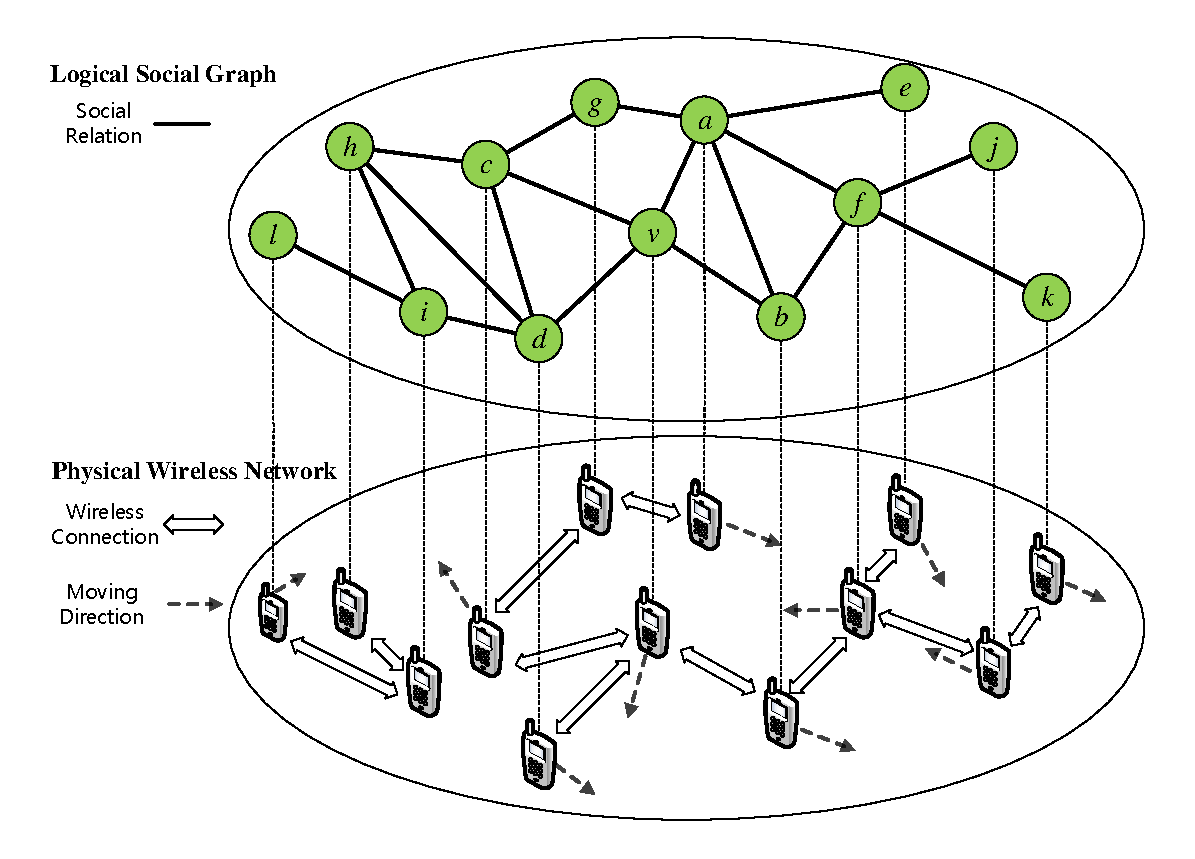
\includegraphics[width=1.05\linewidth]{given2.pdf}
\caption{A wireless network and its social graph}
\label{eego}
\end{figure}

\begin{table}[t]
\center
\caption{Summary of notation}\label{table:symbols}
\small
  \begin{tabular}{| p{0.9cm} | p{6.8cm} |}
    \hline
	Symbol & Description \\  
    \hline
    \hline
	$\V{v}{i}$ & set of $i$-hop neighbors of vertex $v$ ($\V{v}{0} = \{ v \}$)\\
	$\LV{v}{i}$ & set of vertices that are at most $i$ hops away from vertex $v$ (i.e., $\LV{v}{i} = \cup_{k = 0}^{i} \V{v}{k}) $\\
	$\E{v}{i}$ & set of edges connecting a vertex in $\V{v}{i}$ and another vertex in $\V{v}{i}$\\	
	$\LE{v}{i}$ & set of edges connecting a vertex in $\LV{v}{i}$ and another vertex in $\LV{v}{i}$\\
    \hline
  \end{tabular}
\end{table}

In this section, we define terms that represent two types of ego networks of a node in a wireless network (Section~\ref{x-ego_definition}) as well as the betweenness of a node in its ego and x-ego networks (Section~\ref{betweenness}).
We then present several properties of the x-ego networks (Section~\ref{x-go_properties}).
Our betweenness computation algorithm in Section~\ref{computation} takes advantage of these properties.

\subsection{Definitions}\label{x-ego_definition}

% We assume that each DTN node has a fixed transmission range. If two nodes are within range of each other, they are said to be {\em neighbors} \cite{605303}, and a {\em contact} is defined as the status where two nodes are neighbors and can hence exchange data \cite{human_mobility,beyondDTN}. We assume that communication is bidirectional, though it may not be always true in practice due to interference, fades, and hidden nodes.
% 
% To describe our algorithm, we model DTN nodes' relationship as a graph $G(V, E)$, where $V$ is a set of vertices representing the nodes in the DTN and $E$ is a set of unweighted edges representing social links between nodes (see Fig.~\ref{eego} (a))\footnote{Hereinafter, we will use 'vertex' interchangeably with 'node', and 'edge' with 'link'.}. 
% These social links are usually inferred from the sequence of contacts over time in a contact trace. Different metrics such as aggregate contact duration \cite{IEEE:bubble}, contact frequency \cite{4146881,IEEE:bubble} or the age of last contact \cite{Dubois03} have been used to generate such links in the graph.

In this paper, we model a wireless network using a graph $G(V, E)$, where $V$ is a set of vertices representing the nodes in the network and $E$ is a set of edges representing social links between nodes (see Fig.~\ref{eego}).\footnote{We use the term {\em node} and {\em social link} to refer to the devices and their relationships in a wireless network. On the other hand, the graph representing a wireless network consists of {\em vertices} and {\em edges} representing nodes and social links, respectively.}
Given a pair of nodes that have communicated with each other, a social link between these nodes can be assumed if their communications meet certain criteria (e.g., the accumulated duration of communications~\cite{IEEE:bubble}, the frequency of  communications~\cite{4146881,IEEE:bubble}, or the elapsed time after the last communication is beyond/under a threshold~\cite{Dubois03}).
In this paper, we assume undirected social links among nodes (see Section~\ref{data_construction}).
Furthermore, we define the length of a path between two nodes as the number of social links on that path. 
In other words, we model a wireless network using an {\em undirected} and {\em unweighted} graph.

% For a given graph $G(V, E)$ and an arbitrary vertex $v$, let $V_{i}^{v}$ and $E_{i}^{v}$ denote the set of vertices whose shortest distance from $v$ is no larger than $i$ and the set of edges on shortest paths from $v$ to a node in $V_{i}^{v}$, respectively ($V_{0}^{v}=\{v\}$ and $E_{0}^{v}=\emptyset$). For $i\geq1$, the set of $i$-hop neighbors of $v$ is denoted as $N_{i}^{v}(=V_{i}^{v} - V_{i-1}^{v})$. We also denote the set of edges between an $i$-hop neighbor and a $j$-hop neighbor of $v$ as $E_{i \mhyphen j}^{v}$  ($E_{0 \mhyphen 0}^{v}=\emptyset$).
% 
% Using the above terms, a node $v$'s \emph{ego network}~\cite{egocentric,everett,ICCN:lbcdna,SIMBET}, denoted $\EN{v}$, can be defined as follows:
% \begin{definition}\label{def:ego-network}
% Given a graph $G(V, E)$ and a vertex $v \in V$, the \emph{ego network} of $v$ ($\EN{v}$) is the graph consisting of vertex $v$, $v$'s 1-hop neighbors, and the edges between them (i.e., $\EN{v} (V_{1}^{v}$, $E_{1}^{v} \cup E_{1 \mhyphen 1}^{v}$)).
% \end{definition}
% 
% For example, for a network given by Fig.~\ref{eego}~(a) and a vertex $0$, $V_{1}^{0}=\{0,1,2,3,4\}$, $E_{1}^{0}=\{(0,1), (0,2), (0,3), (0,4)\}$, and $E_{1 \mhyphen 1}^{0}=\{(1,2), (3,4)\}$. Therefore, the ego network of $0$ is $\EN{0} (V_{1}^{0}$, $E_{1}^{0} \cup E_{1 \mhyphen 1}^{0})=(\{0,1,2,3,4\}, \{(0,1),(0,2),(0,3),(0,4),(1,2),(3,4)\})$, which is shown in Fig.~\ref{eego}~(b).

In the literature~\cite{egocentric, everett, ICCN:lbcdna, SIMBET}, given a graph $G(V, E)$ and a vertex $v \in V$, the {\em ego network} of $v$ is defined as the subgraph of $G$ consisting of $v$ and its 1-hop neighbors (i.e., vertices with an edge to $v$) as well as the edges between these vertices.
Using the notation summarized in Table~\ref{table:symbols}, this ego network can be formally defined as follows:

\begin{definition}\label{def:ego-network}
Given a graph $G(V, E)$ and a vertex $v \in V$, the \emph{ego network} of $v$ is defined as $\EN{v}(\LV{v}{1}, \LE{v}{1})$ where $\LV{v}{1}$ is the set of vertices whose shortest distance from $v$ is no longer than $1$ (i.e., $\{ v \} \cup \V{v}{1}$) and $\LE{v}{1}$ denotes the set of edges between the vertices in $\LV{v}{1}$.
\end{definition}

\begin{figure}[t]
\centering
\subfigure[Ego network, $\EN{v}$]{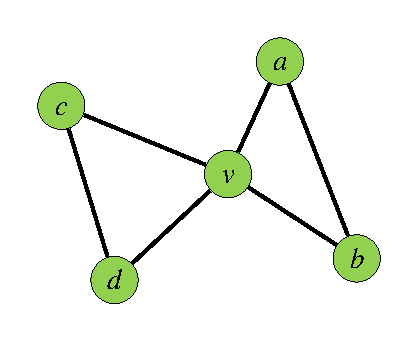
\includegraphics[width=0.36\linewidth]{ego2.pdf}}\label{eego_b}
\subfigure[X-ego network, $\XN{v}$]{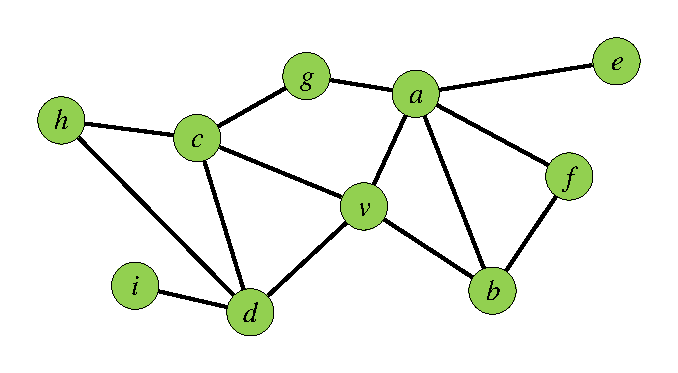
\includegraphics[width=0.6\linewidth]{xego2.pdf}}\label{eego_c}
\caption{Ego and x-ego networks of vertex $v$ in Fig. \ref{eego}}
\label{eego2}
\end{figure} 
\begin{center}
\begin{table*}[t]
 \caption{Comparison of betweenness, ego betweenness, and x-ego betweenness for the graph shown in Fig. \ref{eego} (the Pearson correlation is 0.63 between $\B{v}$ and $\BE{v}$ and 0.90 between $\B{v}$ and $\BX{v}$, and the Spearman correlation is 0.79 between $\B{v}$ and $\BE{v}$ and 0.93 between $\B{v}$ and $\BX{v}$)}\label{comparison}
 \resizebox{17.4cm}{!} {
 \begin{tabular}{|c|c|c|c|c|c|c|c|c|c|c|c|c|c|c|}
 \hline
\multicolumn{2}{|c|}{Nodes} & v & a & b & c & d & e & f & g & h & i & j & k & l \\
 \hline
\multirow{2}{*}{$\B{v}$} & Value & 0.405 & 0.383 & 0.124 & 0.131 & 0.286 & 0.000 & 0.318 & 0.049 & 0.030 & 0.167 & 0.000 & 0.000 & 0.000\\
\hhline{~--------------}
& Rank & 1 & 2 & 7 & 6 & 4 & 10 & 3 & 8 & 9 & 5 & 10 & 10 & 10\\
\hhline{---------------}
\multirow{2}{*}{$\BE{v}$} & Value & 0.667 & 0.750 & 0.167 & 0.583 & 0.333 & 0.000 & 0.833 & 1.000 & 0.167 & 0.667 & 0.000 & 0.000 & 0.000\\
\hhline{~--------------}
& Rank & 4 & 3 & 8 & 6 & 7 & 10 & 2 & 1 & 8 & 4 & 10 & 10 & 10\\
\hhline{---------------}
\multirow{2}{*}{$\BX{v}$} & Value & 0.383 & 0.500 & 0.125 & 0.269 & 0.339 & 0.000 & 0.524 & 0.214 & 0.133 & 0.400 & 0.000 & 0.000 & 0.000\\
\hhline{~--------------}
& Rank & 4 & 2 & 9 & 6 & 5 & 10 & 1 & 7 & 8 & 3 & 10 & 10 & 10\\
\hhline{---------------}
 \hline
 \end{tabular}
}
\end{table*}
\end{center}

\vspace{-10mm}In Fig.~\ref{eego}, $\LV{v}{1} = \V{v}{0} \cup \V{v}{1} = \{v, a, b, c, d\}$ and $\LE{v}{1}=\{ \{v, a\}, \{v, b\}, \{v, c\}, \{v, d\},$ $\{a, b\}, \{c, d\} \}$.
The ego network of vertex $v$, $\EN{v}(\LV{v}{1}, \LE{v}{1})$, is shown in Fig.~\ref{eego2}(a).

% In a DTN, nodes usually broadcast its identifier and resources (such as buffer availability) to all neighboring nodes within their transmission range. These messages sent by a neighbor node $n$ may contain information about its 1-hop neighbors (i.e., $N_{1}^{n}$) to support sophisticated routing protocols \cite{605303,4698820}. A node $v$ receiving $N_{1}^{n}$ from each of its neighbor $n$ (i.e., $n \in {N_{1}^{v}}$) can infer the links between its 1-hop neighbors (i.e., $E_{0 \mhyphen 0}^{v}$), and obtain its ego network.
% 
% For example, assume that a node represented by vertex $0$ in Fig.~\ref{eego} (a) receives information about nodes $N_{1}^{1}=\{0, 2, 5, 6, 7\}$ from node $1$ and information about nodes $N_{1}^{2}=\{0, 1, 6\}$ from node $2$.
% In this case, node $0$ can infer the link represented by the edge between $1$ and $2$.
% Similarly, node $0$ can infer the link between $3$ and $4$ based on messages from $3$ and $4$.
% Then, node $0$ can obtain its ego network $\EN{0} (V_{1}^{v}$, $E_{1}^{0} \cup E_{1 \mhyphen 1}^{0})$.
In a wireless network, the ego network of each node (i.e., the ego network of the vertex representing that node) can be obtained if all of the nodes periodically broadcast information about their neighbors. 
For example, in the wireless network illustrated by Fig.~\ref{eego}, assume that nodes $a$, $b$, $c$, and $d$  broadcast this information and node $v$ has been receiving such information. 
Then, node $v$ will be able to derive its ego network as in Fig.~\ref{eego2}(a).
% It should be noted that the ego network of $v$ does not fully capture the information received from $v$'s neighbors (i.e., misses the links between $v$'s 1-hop and 2-hop neighbors).
% If we fully integrate such information, we obtain the following, which we call {\em eXpanded ego (in short, x-ego) network}:
% \begin{definition}\label{def:xego-network}
% Given a graph $G(V, E)$ and a vertex $v \in V$, the \emph{eXpanded ego (x-ego) network} of $v$ ($\XN{v}$) is the graph consisting of $v$'s 1-hop and 2-hop neighbors, as well as the edges between $v$ and a 1-hop neighbor, between 1-hop and 2-hop neighbors, and between 1-hop neighbors (i.e., $\XN{v} (V_{2}^{v}$, $E_{2}^{v} \cup E_{1 \mhyphen 1}^{v}$)).
% \end{definition}

In the context of wireless networks, ego networks well model the relationships/interactions between a node and others.
However, ego networks have the limitation that it does not capture a substantial amount of information obtained at the expense of network resources.
For example, in Fig.~\ref{eego}, assume that node $v$ received from node $a$ the information about $a$'s 1-hop neighbors (i.e., $b$, $e$, $f$, $g$, and $v$).
Despite this information, the ego network of $v$ cannot record the social links between $a$ and $e$, between $a$ and $f$, and between $a$ and $g$ since it can represent only the social links between $v$ and the 1-hop neighbors of $v$.

To overcome the above limitation, we introduce the following extension to ego networks:

\begin{definition}\label{def:xego-network}
Given a graph $G(V, E)$ and a vertex $v \in V$, the \emph{extended ego network} (briefly, \emph{x-ego network}) of $v$ is $\XN{v} (\LV{v}{2}, \LE{v}{2} - \E{v}{2})$, where $\LV{v}{2}$ is the set of vertices that are at most 2 hops away from $v$, $\LE{v}{2}$ is the set of edges between vertices that are at most 2 hops away from $v$, and $\E{v}{2}$ is the set of edges between 2-hop neighbors of $v$.
\end{definition}

% For example, the x-ego network of the node represented by vertex 0 is  $\XN{0} (V_{2}^{0}$, $E_{2}^{0} \cup E_{1 \mhyphen 1}^{0})$ shown in Fig.~\ref{eego} (c). x-ego networks are different from 2nd order ego networks (or friends of friends) of which edge sets includes $E_{2 \mhyphen 2}^{v}$ as well as $E_{2}^{v} \cup E_{1 \mhyphen 1}^{v}$. 
% 
% Note that the vertex and edge sets of an x-ego network $\XN{v}$ for a vertex $v$ are also defined as follows:
% \begin{eqnarray}\label{chi}
% V_{2}^{v} &=& \bigcup_{n \in N_{1}^{v}} V_{1}^{n},\\
% E_{2}^{v} \cup E_{1 \mhyphen 1}^{v} &=& \bigcup_{n \in N_{1}^{v}} E_{1}^{n}.
% \end{eqnarray} It means that a vertex $v$ can generate its x-ego network by using the neighbor information of its neighbors. In summary, both ego and x-ego networks can be obtained with the same (similar) network overhead.
% However, expanded ego networks inherently contain substantially larger amounts of information than ego networks.
% As experimentally demonstrated in Section~\ref{experiments}, highly accurate betweenness centrality values can be obtained from x-ego networks than ego networks.

Fig.~\ref{eego2}(b) shows the x-ego network of $v$ from the graph in Fig.~\ref{eego}.
As Fig.~\ref{eego2}(a) and Fig.~\ref{eego2}(b) illustrate, the x-ego network of $v$ is different from the ego network of $v$ in that it contains 2-hop neighbors of $v$ (i.e., $\LV{v}{2} - \LV{v}{1} = \V{v}{2}$) as well as the edges between a 1-hop neighbor and a 2-hop neighbor of $v$.
Despite this difference, both the ego and x-ego networks of $v$ can be obtained with the same network overhead (since they consume the same messages from 1-hop neighbors of $v$).
The benefits of x-ego networks over ego networks are further verified in Section~\ref{evaluation}.

% For a given graph $G(V, E)$ and an arbitrary vertex $v$, we define the following terms:
% \begin{itemize}
% \item $V_{i}^{v}$: the set of vertices whose shortest distance from $v$ is no larger than $i$ (hence, $V_{0}^{v}=\{v\}$).
% \item $E_{i}^{v}$: the set of edges on shortest paths from $v$ to a node in $V_{i}^{v}$ (hence, $E_{0}^{v}=\emptyset$).
% \item $E_{i \mhyphen j}^{v}$: the set of edges between an $i$-hop neighbor and a $j$-hop neighbor of $v$ (hence, $E_{0 \mhyphen 0}^{v}=\emptyset$).
% \item $N_{i}$: the set of 1-hop neighbor nodes with a direct link to $v_i$.
% \item $E_{i}$: the set of links between $v_i$ to the nodes in $N_{i}$.
% \item $\bar{E}_{i}$: the set of links among the nodes in $N_{i}$.
% \end{itemize} 

%The ego network model has been frequently used in many network analysis. The ego network is the network consisting of a single node(ego) together with the 1st-hop neighbor nodes they are connected to and all the links among those neighbors.
% We also define the following additional terms:
% \begin{itemize}
% \item $N^{2}_{i}$: the set of $v_i$'s 2-hop neighbor nodes each of which has a direct link to a node in $N_{i}$.
% \item $E^{2}_{i}$: the set of links connecting the $N_{i}$ nodes to the $N^{2}_{i}$ nodes.
% %\item $\ddot{E}_{N^{2}_{i}}$: the set of edges of nodes belong to $N^{2}_{i}$.
% \end{itemize} 

\subsection{Ego and X-Ego Betweenness}\label{betweenness}

% In much literature, the betweenness $C_{B}(i)$ for a node $v$ has been formally defined as follows:\begin{equation}\label{bet}
% C_{B}(v) = \frac{\sum_{s \neq v \neq t \in V, s<t}\frac{\sigma_{st}(v)}{\sigma_{st}}}{(n-1)(n-2)/2}.
% \end{equation} where $n$ is the total number of nodes, $\sigma_{st}$ is the number of shortest paths from $s$ to $t$, and $\sigma_{st}(i)$ is the number of those shortest paths that include the node $v$. In an undirected network, $\sigma_{st}=\sigma_{ts}$ and $\sigma_{st}(i)=\sigma_{ts}(i)$. The denominator denotes the total number of pairs of nodes except $v$ in an undirected network and normalizes $C_{B}(v)$ to a value between 0 and 1.

In the literature~\cite{centrality, everett, Brandes01afaster}, given a graph $G(V, E)$, the betweenness $\B{v}$ of a vertex $v$ is defined as:
\begin{equation}\label{bet}
\B{v} = \frac{\sum_{s \neq v \neq t \in V}\frac{\sigma_{st}(v)}{\sigma_{st}}}{(|V|-1)(|V|-2)}
\end{equation} where $\sigma_{st}$ is the number of shortest paths from vertex $s$ to vertex $t$ and $\sigma_{st}(v)$ is the number of those shortest paths that pass through vertex $v$. 
% \B{v} = \frac{2 \cdot \sum_{s \neq v \neq t \in V,\ s < t}\frac{\sigma_{st}(v)}{\sigma_{st}}}{(|V|-1)(|V|-2)}.
% \end{equation} where $\sigma_{st}$ is the number of shortest paths from vertex $s$ to vertex $t$ and $\sigma_{st}(v)$ is the number of those shortest paths that pass through vertex $v$. 
In the above definition, the denominator represents the total number of pairs of vertices except $v$.
It normalizes $\B{v}$ to a value between 0 and 1.
Given an undirected graph, $\sigma_{st}=\sigma_{ts}$ and $\sigma_{st}(v)=\sigma_{ts}(v)$ for all vertices $s$, $t$, and $v$.
Therefore, it is sufficient to find either $\sigma_{st}$ or $\sigma_{ts}$ and either $\sigma_{st}(v)$ or $\sigma_{ts}(v)$.

% The globally computed betweenness based on (\ref{bet}) requires much information about the whole network topology and causes large computational and message load overheads. Since a DTN node may be energy-constrained and there is usually no explicit centralized network node in a DTN, such computation is not reasonable. Thus, getting local information from encounter nodes and generating ego or x-ego networks in a distributed way are practically feasible.
% 
% A node $v$'s \emph{ego betweenness} $C^{\mathcal{E}}_{B}(v)$ on its ego network $\EN{v}$ is locally computed as follows:\begin{equation}\label{ebet}
% C^{\mathcal{E}}_{B}(v) = \frac{\sum_{s \neq v \neq t \in V_{1}^{v}, s<t}\frac{\sigma_{st}(v)}{\sigma_{st}}}{(|V_{1}^{v}|-1)(|V_{1}^{v}|-2)/2}. 
% \end{equation} and the \emph{x-ego betweenness} $C^{\mathcal{X}}_{B}(v)$ on its x-ego network $\XN{v}$ is also locally obtained as follows: \begin{equation}\label{eebet}
% C^{\mathcal{X}}_{B}(v) = \frac{\sum_{s \neq v \neq t \in V_{2}^{v}, s<t}\frac{\sigma_{st}(v)}{\sigma_{st}}}{(|V_{2}^{v}|-1)(|V_{2}^{v}|-2)/2}.
% \end{equation} Although the x-ego betweenness requires more computational time than the ego betweenness, it has the similar benefit of simplicity with the ego network in terms of information collection and network configuration. On the other hand, the x-ego betweenness includes more local information than the ego network, so that it will be more accurate than the ego betweenness. 

In a large wireless network, obtaining the betweenness of each node (i.e., the betweenness of the vertex representing that node) is costly since  all nodes that have limited memory and energy must exchange and consume a substantial number of messages to identify the shortest paths between them.
On the other hand, each node can obtain its ego and x-ego networks with much lower overhead since each node  needs to broadcast information about its 1-hop neighbors (Section~\ref{x-ego_definition}). 
In this paper, we consider the situations where each node computes its betweenness using either its ego network or x-ego network and then uses the result as an estimate of its true betweenness in the entire network.
We refer to the betweenness of $v$ computed from the ego network and x-ego network of $v$ as the {\em ego betweenness} and {\em x-ego betweenness} of $v$ (denoted $\BE{v}$ and $\BX{v}$), respectively.

% To compare the accuracy of $\BE{v}$ or $\BX{v}$, we first use the Spearman's rank correlation which measures the {\em monotonic} relationship between the ranked variables of $\BX{v}$ and $\B{v}$ or $\BE{v}$ and $\B{v}$.  The correlation value can vary between -1.0 and +1.0. The closer value is to +1.0, the stronger the association between the values. For the sake of completeness, we also measure the well-known Pearson correlation. The Pearson correlation coefficient assesses a {\em linear} relationship between the two variables and the calculation is based not on the ranked variables, but on the actual betweenness values.

% For the networks shown in Fig. \ref{}, Table \ref{comparison} shows the comparison of globally computed, ego, and x-ego betweenness. Although the actual betweenness values are different with each other, we can see that 1) the rank order of the three betweenness values are very similar to each other, and 2) the rank order of x-ego betweenness is more similar to the one of globally computed betweenness than the one of ego betweenness. We will verify the details with real mobility trace data in Section IV.

Table~\ref{comparison} shows, for every vertex $v$ in Fig.~\ref{eego}, the betweenness ($\B{v}$), ego betweenness ($\BE{v}$), and x-ego betweenness ($\BX{v}$).
In this table, for most of the vertices, x-ego betweenness is closer to betweenness than ego-betweenness mainly because it is derived from a larger number of vertices and edges.
For this reason, the correlation coefficient (also known as the Pearson correlation coefficient) of x-ego betweenness and betweenness (0.9) is higher than that of ego-betweenness and betweenness (0.63).
The advantage of x-ego betweenness over ego betweenness can also be observed in terms of Spearman's rank correlation, which indicates, given two series $\mathcal{X}=(X_1, X_2, \cdots, X_N)$ and $\mathcal{Y}=(Y_1, Y_2, \cdots, Y_N)$, the correlation between $(r_{\mathcal{X}}(X_1), r_{\mathcal{X}}(X_2)$ $, \cdots, r_{\mathcal{X}}(X_N))$ and $(r_{\mathcal{Y}}(Y_1), r_{\mathcal{Y}}(Y_2), \cdots, r_{\mathcal{Y}}(Y_N))$, where $r_{\mathcal{X}}(X_i)$ and $r_{\mathcal{Y}}(Y_i)$ represent the rank of $X_i$ in $\mathcal{X}$ and that of $Y_i$ in $\mathcal{Y}$, respectively.
In Table~\ref{comparison}, Spearman's correlation is 0.93 between x-ego betweenness and betweenness and 0.79 between ego betweenness and betweenness.
In Section~\ref{evaluation}, we further demonstrate the benefit of x-ego betweenness using wireless trace data.

\subsection{Properties of X-Ego Networks}\label{x-go_properties}
In this section, we present four properties of x-ego networks. 
These properties enable efficient x-ego betweenness computation (Section~\ref{computation}). 
As in Brandes' work~\cite{Brandes01afaster}, we denote the \emph{dependency} of vertices $s$ and $t$ on vertex $v$ as $\D{s}{t}{v} = \frac{\sigma_{st}(v)}{\sigma_{st}}$.
Then, the betweenness of $v$ (Equation (\ref{bet})) can be computed by adding the dependency values for all pairs of vertices excluding $v$.
To quickly calculate such dependency values in x-ego networks, we have identified the properties explained below. 

% By Equation (\ref{bet}), we can know that the betweenness of $v$ can be obtained by summing the dependencies for all pairs of vertices, except for $v$, in $\XN{v}$.
% % The exhaustive search of such all shortest paths is computationally expensive. 
% We identify the following properties, {\em Theorem \ref{theorem1}, \ref{theorem2}, \ref{theorem3}}, and  {\em \ref{theorem4}}, to obtain such dependencies with low computational overhead.
% % Therefore, we need to devise {\em skip conditions} or (\ldots) to reduce the computational burden.  
\begin{theorem}
\label{theorem1} 
Assume a vertex $v$, its x-ego network $\XN{v}$, and its two different 1-hop neighbors $s$ and $t$ (i.e., $s, t \in \V{v}{1}$ and $s \ne t$).
Then, $\D{s}{t}{v} = 0$ if there is an edge between $s$ and $t$ (i.e., $\{s, t\} \in \E{v}{1}$).
\begin{proof}
Since $\{s, t\} \in \E{v}{1}$, $d(s, t) = 1$.
Furthermore, $s, t \in \V{v}{1}$, meaning that $d(s, v) + d(v, t) = 1 + 1 = 2 > d(s, t) = 1$ (i.e., no shortest path from $s$ to $t$ passes through $v$).
Therefore, $\D{s}{t}{v} = \sigma_{st}(v)/\sigma_{st} = 0/\sigma_{st} = 0$.\hfill\qed
\end{proof}
\end{theorem}


\begin{example}
In Fig.~\ref{eego2}(b), $\D{a}{b}{v} = 0$ since $a, b \in \V{v}{1}$ and there is an edge between $a$ and $b$.
\end{example}

% Theorem \ref{theorem1} will take on a key role as a computation skipping rule in the algorithm to compute the x-ego betweenness, $\BX{v}$. In particular, it will reduce the computational overload substantially when a vertex $v$'s x-ego network exhibits a strong community structure (i.e., nodes in ego networks tend to interact with each other). Since friends of a friend are likely to be friends as well, we can expect that this transitivity should be frequently observed in x-ego networks derived by a DTN. 
% 
% In case that the skipping rule presented by Theorem \ref{theorem1} cannot be applied for a pair of $v$'s two 1-hop neighbors, the dependency of them is computed by using the following Theorem \ref{theorem2}. 

Theorem \ref{theorem1} allows us to quickly compute dependencies particularly when x-ego networks exhibit a strong community structure (i.e., 1-hop neighbors of a node tend to have direct social links between them).
In Section~\ref{evaluation}, we show this benefit using wireless trace data.

When Theorem \ref{theorem1} cannot be applied to $v$'s 1-hop neighbors $s$ and $t$ (i.e., there is no edge between $s$ and $t$), the dependency of $s$ and $t$ on $v$ can be computed using the following theorem.

\begin{theorem}
\label{theorem2} 
Assume a vertex $v$, its x-ego network $\XN{v}$, and its two different 1-hop neighbors $s$ and $t$ (i.e., $s, t \in \V{v}{1}$ and $s \ne t$).
Then, $\D{s}{t}{v} = {1}/{|\V{s}{1} \cap \V{t}{1}|}$ if there is no edge between $s$ and $t$ (i.e., $\{s, t\} \notin \E{v}{1}$).
\begin{proof}
Since $\{s, t\} \notin \E{v}{1}$, $d(s, t) > 1$.
In this case, $d(s, t) = 2$ due to the path $s - v - t$.
Furthermore, (i) the number of shortest paths from $s$ to $t$ (i.e., paths whose length is 2) can be expressed as $\sigma_{st} = |\V{s}{1} \cap \V{t}{1}|$.
%  indicates the number of shortest paths starting from $v_s \in N_0$ and terminating at $v_t \in N_0$.
On the other hand, (ii) the path $s-v-t$ is the only shortest path from $s$ to $t$ that passes through $v$ (i.e., $\sigma_{st}(v) = 1$) since the length of that path is 2, which must be smaller than the length of any other path from $s$ to $t$ that passes through $v$.
By (i) and (ii), $\D{s}{t}{v} = \sigma_{st}(v)/\sigma_{st} = {1}/{|\V{s}{1} \cap \V{t}{1}|}$.\hfill\qed
\end{proof}
\end{theorem}

% \begin{equation}
% \D{s}{t}{v} =
%   \begin{cases}
%    0       & \text{if $(s, t) \in E$} \\
%    {\displaystyle \frac {1}{|\V{s}{1} \cap \V{t}{1}|}} & \text{ otherwise.} \\
%   \end{cases}
% \end{equation}

\begin{example}
\label{example2} 
In Fig.~\ref{eego2}(b), vertices $a$ and $c$ are 1-hop neighbors of $v$ and there is no edge between $a$ and $c$.
Furthermore, $\V{a}{1} = \lbrace b, e, f, g, v\rbrace$ and $\V{c}{1} = \lbrace d, g, h, v\rbrace$.
Therefore, $\D{a}{c}{v}=1/|\V{a}{1} \cap \V{c}{1}|=1/|\{g, v \}|=1/2$.

% $\LV{a}{1} = \lbrace v, b, e, f, g\rbrace$, $\LV{c}{1} = \lbrace v, d, g, h\rbrace$ and $\LV{d}{1} = \lbrace v, c, h, i\rbrace$. So, node $v$ can get the non-zero $\D{a}{c}{v}=1/2=0.5$ and $\D{a}{d}{v}=1/1=1$ because $v$ knows that $a$ does not share any edge with $c$ and $d$, $|\LV{a}{1} \cap \LV{c}{1}| = |\lbrace v, g\rbrace|=2$, and $|\LV{a}{1} \cap \LV{d}{1}| = |\lbrace v\rbrace$| = 1. 
\end{example}

Just like Theorem~\ref{theorem1}, the following theorem quickly computes the dependency of two vertices on a vertex $v$.
While the former applies to a pair of 1-hop neighbors of $v$, the latter applies to a pair of a 1-hop or 2-hop neighbor and a 2 hop-neighbor of $v$.
% The following Theorem \ref{theorem3} presents another skipping rule to reduce the computation overload of the dependency for an 1 or 2-hop neighbor and a 2-hop neighbor of $v$.

\begin{theorem}
\label{theorem3} 
Assume a vertex $v$, its x-ego network $\XN{v}$, a vertex $s \in \LV{v}{2}$, and another vertex $t \in \V{v}{2}$ such that $s \ne t$.
Then, $\D{s}{t}{v} = 0$ if $\D{s}{n}{v} = 0$ for a 1-hop neighbor vertex $n$ of vertex $t$ (i.e., for $n \in \V{t}{1}$).
\begin{proof}
Since $\D{s}{n}{v} = 0$ (i.e., no shortest path from $s$ to $n$ passes through $v$), (i) $d(s, n) < d(s, v) +d(v, n)$.
Then, (ii) $d(s, t) \le d(s, n) + d(n, t) < d(s, v) + d(v, n) + d(n, t)$ by (i).
Furthermore, $n \in \V{t}{1}$ and $t \in \V{v}{2}$, meaning that vertex $n$ is either a 1-hop or a 3-hop neighbor of $v$.
In $\XN{v}$, however, any vertex including $n$ is at most 2 hops away from $v$.
For this reason, $n$ is a 1-hop neighbor of $v$.
Since $d(v, n)$=$d(n, t)$=$1$ and $d(v, t)=2$, (iii) $d(v, n) + d(n, t) = d(v, t)$. 
By (ii) and (iii), $d(s, t) < d(s, v) +d(v, t)$ (i.e., no shortest path from $s$ to $t$ passes through $v$).
Therefore, $\D{s}{t}{v}  = \sigma_{st}(v)/\sigma_{st} = 0/\sigma_{st} = 0$.\hfill\qed
\end{proof}
\end{theorem}

\begin{example}
In Fig. \ref{eego2}(b), $b \in \LV{v}{2}$ and $g \in \V{v}{2}$. 
Furthermore, for a 1-hop neighbor $a$ of $g$, $\D{b}{a}{v}=0$ (Theorem \ref{theorem1}).
Therefore, by Theorem \ref{theorem3}, $\D{b}{g}{v}=0$.
\end{example}

Given vertices $s \in \LV{v}{2}$ and $t \in \V{v}{2}$ such that $s \ne t$, Theorem~\ref{theorem3} cannot be applied if $\D{s}{n}{v} > 0$ for every 1-hop neighbor $n$ of $t$.
In this case, the dependency of $s$ and $t$ on $v$ can be obtained using the following theorem.
% Lastly, the following Theorem \ref{theorem4} presents that the harmonic mean can be used to compute the dependency for an 1 or 2-hop neighbor and a 2-hop neighbor of $v$, if they do not satisfy the condition of Theorem \ref{theorem3}. 

\begin{theorem}
\label{theorem4} 
Assume a vertex $v$, its x-ego network $\XN{v}$, a vertex $s \in \LV{v}{2}$, and another vertex $t \in \V{v}{2}$ such that $s \ne t$.
Then, $\D{s}{t}{v} = \bar{H}(\{\D{s}{n}{v} : n \in \V{t}{1}\})$ if $\D{s}{n}{v} > 0$ for every 1-hop neighbor $n$ of vertex $t$, where $\bar{H}(\{\D{s}{n}{v} : n \in \V{t}{1}\})$ denotes the {\em harmonic mean} computed over $\{\D{s}{n}{v} : n \in \V{t}{1}\}$.
\begin{proof}
We prove this theorem considering the following two cases.
% in two cases, $s \in \LV{v}{1}$ or $s \in \LV{v}{2}-\LV{v}{1}$, separately:

\noindent [Case I. $s$ is a 1-hop neighbor of $v$ (i.e., $s \in \V{v}{1}$)]
% Let us assume there are $m$ 1-hop neighbors of $t$ in $\XN{v}$ and let $n_i$ denote the $i$th 1-hop neighbor of $t$ such that $\D{s}{n_i}{v} > 0$. In $\XN{v}$, each $n_i$ is also an 1-hop neighbor of $v$ (i.e., $n_i \in \LV{v}{1}$) and $\D{s}{n_i}{v} = {1}/{|\LV{s}{1} \cap \LV{n_i}{1}|}$ by Theorem \ref{theorem2}. 
% Furthermore, (i) $|\LV{s}{1} \cap \LV{n_i}{1}|=1/\D{s}{n_i}{v}$ represents the number of shortest paths from $s$ to $n_i$ (i.e., $\sigma_{sn_i}$) and the total number of shortest paths from $s$ to $t$ can be expressed as $\sigma_{st} = \sum_{i=1}^m 1/\D{s}{n_i}{v}$ since each $n_i$ shares an edge with $t$. On the other hand, (ii) the path $s-v-n_i-t$ is the only shortest path from $s$ to $t$ via both $v$ and $n_i$ since the length of the path is 3 and any other path from $s$ to $t$ via both $v$ and $n_i$ must be longer. It means that there are $m$ shortest paths from $s$ to $t$ via $v$ (i.e., $\sigma_{st}(v)=m$). By (i) and (ii), $\D{s}{t}{v} = \frac{m}{\sum_{i=1}^m 1/\D{s}{n_i}{v}} = \bar{H}(\D{s}{n}{v})$.
Let $n_i$ ($i=1,2,\cdots, m$) denote the $i$th 1-hop neighbor of $t$.
Then, each $n_i$ is a 1-hop neighbor of $v$ since, in $\XN{v}$, any 2-hop neighbor (including $t$) of $v$ can be connected only to a 1-hop neighbor of $v$ (Definition~\ref{def:xego-network}).
Thus, by Theorem \ref{theorem2}, $\D{s}{n_i}{v} = {1}/{|\V{s}{1} \cap \V{n_i}{1}|}$. 
Since $|\V{s}{1} \cap \V{n_i}{1}|$ represents the number of shortest paths from $s$ to $n_i$ (i.e., $\sigma_{sn_i}$) and each $n_i$ has an edge to $t$, the total number of shortest paths from $s$ to $t$ can be expressed as (i) $\sigma_{st} = \sum_{i=1}^m |\V{s}{1} \cap \V{n_i}{1}| = \sum_{i=1}^m 1/\D{s}{n_i}{v}$. 
On the other hand, the path $s-v-n_i-t$ is the only shortest path from $s$ to $t$ via both $v$ and $n_i$ since the length of the path is 3 and any other path from $s$ to $t$ via both $v$ and $n_i$ must be longer.
For this reason, (ii) there are $m$ shortest paths from $s$ to $t$ via $v$ (i.e., $\sigma_{st}(v)=m$).
By (i) and (ii), $\D{s}{t}{v} = \frac{m}{\sum_{i=1}^m 1/\D{s}{n_i}{v}} = \bar{H}(\D{s}{n}{v})$.

\noindent [Case II. $s$ is a 2-hop neighbor of $v$ (i.e., $s \in \V{v}{2}$)]
Let $n_i~(i=1,2,\cdots,m)$ denote the $i$th 1-hop neighbor of $t$. 
Let also $p_j~(j=1,2,\cdots,k)$ denote the $j$th 1-hop neighbor of $s$.
In $\XN{v}$, 2-hop neighbors (including $s$ and $t$) of $v$ can be connected only to a 1-hop neighbor of $v$.
For this reason, any shortest path from $s$ to $t$ must contain a shortest path from $p_j$ to $n_i$ for some $j$ and $i$ 
% Since $n_i$ and $p_j$ respectively shares an edge with $t$ and $s$, the shortest path from $n_i$ to $n_j$ for a pair of $i$ and $j$ always corresponds to the one from $s$ to $t$ 
(i.e., $\sigma_{st} = \sum_{i=1}^m \sum_{j=1}^k |\V{n_i}{1} \cap \V{p_j}{1}|$). 
For a pair of $i$ and $j$, on the other hand, the path $n_i-v-p_j$ is the only shortest path from $n_i$ to $p_j$ via $v$ and so is the path $t-n_i-v-p_j-s$ (i.e., $\sigma_{st}(v)=mk$). 
Therefore, 
\begin{eqnarray}
\D{s}{t}{v} 
&=& \frac{mk}{\sum_{i=1}^m \sum_{j=1}^k |\V{n_i}{1} \cap \V{p_j}{1}|} \nonumber \\ 
&=& \frac{mk}{\sum_{i=1}^m \sum_{j=1}^k 1/\D{n_i}{p_j}{v}} \nonumber \\ 
&=& \frac{m}{\sum_{i=1}^m \frac {\sum_{j=1}^k 1/\D{n_i}{p_j}{v}}{k}} \nonumber \\ 
&=& \frac{m}{\sum_{i=1}^m 1/\D{n_i}{s}{v}} \nonumber \\ 
&=& \frac{m}{\sum_{i=1}^m 1/\D{s}{n_i}{v}} \nonumber  \\
&=& \bar{H}(\D{s}{n}{v}).   \nonumber
\end{eqnarray}\qed
\label{harmonic_eq}
\end{proof}
\end{theorem}

% \label{harmonic} 
% For a vertex $v$, its x-ego network $\XN{v}$, a vertex $s \in \V{v}{1} \cup \V{v}{2}$ and another vertex $t \in \V{v}{2}$, let $n_1, n_2, \cdots, n_i$ ($n_i \leq u$) denote the 1-hop neighbor vertices of vertex $t$. 
% Then, 
% \begin{equation}
% \D{s}{t}{v} =
%   \begin{cases}
%    0      &\text{if $\exists k, \D{s}{n_k}{v} = 0$} \\
%    \bar H (\D{s}{n_k}{v}) &\text{otherwise.}
%    \end{cases}
% \end{equation} where $\bar H_{st}$ is the harmonic mean for all the non-zero $f_{s{n_k}}$ values.
% \end{theorem}
% \begin{proof}
% ...\\
% ...\\
% ...\\
% ... \qed
% \end{proof}
\begin{example}
In Fig.~\ref{eego2}(b), % consider the dependency $\D{a}{h}{v}$ of $a \in \LV{v}{2}$ and $h \in \V{v}{2}$ on $v$. In this example, 
$\V{h}{1} = \{c,d\}$.
By Theorem \ref{theorem2}, $\D{a}{c}{v}=\frac{1}{2}$ and $\D{a}{d}{v}=1$.
Therefore, by Theorem \ref{theorem4}, $\D{a}{h}{v}\!=\!\bar{H}(\{\D{a}{n}{v} : n \in \V{h}{1}\})\!=\!\bar{H}(\{\D{a}{c}{v},\D{a}{d}{v}\})\!=\!\frac{2}{\frac{1}{\frac{1}{2}} + \frac{1}{1}}=\frac{2}{3}$.  
 
% For each 1-hop neighbor $n$ of $h$ (i.e., $n \in \V{h}{1} = \{ c,d\}$,  and from Theorem \ref{theorem2} it also knows $\D{a}{c}{v}=1/2$ and $\D{a}{d}{v}=1/1$ for $h$'s two 1-hop neighbors, $c$ and $d$. Therefore, we can get $\D{a}{h}{v}$=$\bar{H}(\D{a}{c}{v},\D{a}{d}{v})$=$2/3$. 
% Similarly, $\D{c}{e}{v}=\bar{H}(\D{c}{a}{v})=1/2$ where $c \in \LV{v}{1} (\subset \LV{v}{2})$ and $e \in \LV{v}{2}-\LV{v}{1}$, since $\LV{e}{1}=\{e,a\}$, $\D{c}{a}{v}=1/2$ and $\bar{H}(\D{c}{a}{v})=\D{c}{a}{v}$.
\end{example}

% These four properties will be used in the algorithm proposed in Section \ref{computation} to compute the x-ego betweenness of a DTN node.

\section{X-ego Betweenness Computation}\label{computation}

This section provides an overview of previous work on betweenness computation (Section~\ref{brandes}), presents our algorithm for quickly computing x-ego betweenness (Section~\ref{algorithm}), and analytically shows the benefits of our algorithm (Section~\ref{discussion}).

\subsection{Previous Work on Betweenness Computation}\label{brandes}
% Due to the small number of nodes in x-ego networks compared to the one in the global network, the x-ego betweenness will be computed faster than globally computed betweenness. But, some nodes can have a large number of 1-hop and 2-hops neighbor nodes and the calculation of shortest paths between all pairs of such nodes can be still computationally expensive. So, we propose a fast scheme to compute the x-ego betweenness in this section.
% Brandes \cite{Brandes01afaster} presents a fast algorithm, called \emph{Brandes}, to compute the betweenness of each vertex in a given graph.
To the best of our knowledge, the fastest algorithm for computing the betweenness of every vertex in a given graph is developed by Brandes~\cite{Brandes01afaster}.
%It is based on solving a single source shortest path problem (SSSP) from each vertex. 
Given an unweighted graph, this algorithm performs breadth first search from each vertex to compute the number of shortest paths from that vertex (i.e., the root of search) to each visited vertex.
% Such path computation from a vertex produces a directed acyclic graph (DAG) encoding all shortest paths starting at the vertex. 
% By backward aggregation of counter values, the contributions of these paths to the betweenness can be computed in linear time. 
The Brandes algorithm then derives the betweenness of each vertex by aggregating the previously computed count values backwards along the edges.
% By backward aggregation of counter values, the contributions of these paths to the betweenness can be computed in linear time. 
% The algorithm takes time between $O(VE)$ time for unweighted graphs. 
Given an unweighted graph $G(V, E)$, this Brandes algorithm takes $O(|V| |E|)$ time.
% Although this is polynomial time, it is still prohibitive for networks with many number of vertices and edges.
% Bader and Madduri \cite{bader06centrality} present a parallel implementation of the algorithm that can handle a few million nodes.

% It is worth noting that the Brandes algorithm tries to compute the betweenness of all vertices in a given graph. 
% This is a drawback of getting betweenness values in x-ego networks, since we are interested in the betweenness of a particular vertex in x-ego network.
The x-ego betweenness of a vertex can be found by obtaining the betweenness of that single vertex in the corresponding x-ego network.
Applying the Brandes algorithm to the x-ego network, however, results in finding the betweenness of every vertex in the x-ego network (i.e., the Brandes algorithm incurs overhead to find unneeded information).
% In this section, we hence propose an efficient algorithm to get the betweenness of a given vertex based on theorems in the previous section, which is suitable for computing the x-ego betweenness in x-ego networks. 
% We are currently not aware of any previous work that more quickly computes the betweenness of a vertex than the Brandes algorithm.
Section~\ref{algorithm} presents our algorithm that quickly computes x-ego betweenness by computing the betweenness of only the target vertex and by skipping computations according to the properties of x-ego networks explained in Section~\ref{x-go_properties}.

\subsection{Our X-Ego Betweenness Algorithm}\label{algorithm}

\begin{table}
\caption{Dependency table for vertex $v$ in Fig.~\ref{eego2}(b)}\label{dependency_table}
\begin{center}
\resizebox{8.3cm}{!} {
\renewcommand{\arraystretch}{1.4}
\begin{tabular}{|c|c|c|@{}cccc@{}|@{}ccccc@{}|}
 \hline
 \hline
\multicolumn{3}{|c|}{vertex group} & \multicolumn{4}{|c|}{$\V{v}{1}$} & \multicolumn{5}{|c|}{$\V{v}{2}$} \\ 
\hline
\multirow{2}{*}{mapping $I$} &
\multicolumn{2}{|c|}{vertex} & $a$ & $b$ & $c$ & $d$ & $e$ & $f$ & $g$ & $h$ & $i$ \\ 
%\hline
& \multicolumn{2}{|c|}{index} & 1 & 2 & 3 & 4 & 5 & 6 & 7 & 8 & 9 \\ 
\hline
\multirow{4}{*}{$\V{v}{1}$} & $a$ & 1 & 0 & \normalsize{\bf 0} & \normalsize{\bf 1/2} & \normalsize{\bf 1/1} & \normalsize{\bf 0} & \normalsize{\bf 0} & \normalsize{\bf 0} & \normalsize{\bf 2/3} & \normalsize{\bf 1/1} \\
& $b$ & 2 & 0 & 0 & \normalsize{\bf 1/1} & \normalsize{\bf 1/1} & \normalsize{\bf 0} & \normalsize{\bf 0} & \normalsize{\bf 0} & \normalsize{\bf 2/2} & \normalsize{\bf 1/1} \\
& $c$ & 3 & 1/2 & 1/1 & 0 & \normalsize{\bf 0} & \normalsize{\bf 1/2} & \normalsize{\bf 2/3} & \normalsize{\bf 0} & \normalsize{\bf 0} & \normalsize{\bf 0} \\
& $d$ & 4 & 1/1 & 1/1 & 0 & 0 & \normalsize{\bf 1/1} & \normalsize{\bf 2/2} & \normalsize{\bf 0} & \normalsize{\bf 0} & \normalsize{\bf 0} \\
 \hline
\multirow{5}{*}{$\V{v}{2}$} & $e$ & 5 & 0 & 0 & 1/2 & 1/1 & 0 & \normalsize{\bf 0} & \normalsize{\bf 0} & \normalsize{\bf 2/3} & \normalsize{\bf 1/1} \\
& $f$ & 6 & 0 & 0 & 2/3 & 2/2 & 0 & 0 & \normalsize{\bf 0} & \normalsize{\bf 4/5} & \normalsize{\bf 2/2} \\
& $g$ & 7 & 0 & 0 & 0 & 0 & 0 & 0 & 0 & \normalsize{\bf 0} & \normalsize{\bf 0} \\
& $h$ & 8 & 2/3 & 2/2 & 0 & 0 & 2/3 & 4/5 & 0 & 0 & \normalsize{\bf 0} \\
& $i$ & 9 & 1/1 & 1/1 & 0 & 0 & 1/1 & 2/2 & 0 & 0 & 0 \\
 \hline
 \hline         
\end{tabular}
}
\end{center}
\end{table}

%\begin{table}[t]
%\caption{Neighbor table of node $0$}\label{neighbor_table}
%\begin{center}
%\renewcommand{\arraystretch}{1.3}
%\begin{tabular}{|c|c|}
%\hline
%\hline
%$k \in \V{0}{1} \cup \V{0}{2}$ & $\V{k}{1}$ \\
%\hline
%$1$ & $\{ 0, 2, 5, 6, 7\}$ \\
%\hline
%$2$ & $\{ 0, 1, 6 \}$ \\
%\hline
%$3$ & $\{ 0, 4, 7, 8 \}$ \\
%\hline
%$4$ & $\{ 0, 3, 8, 9 \}$ \\
%\hline
%$5$ & $\{ 1 \}$ \\
%\hline
%$6$ & $\{ 1, 2 \}$ \\
%\hline
%$7$ & $\{ 1, 3 \}$ \\
%\hline
%$8$ & $\{ 3, 4 \}$ \\
%\hline
%$9$ & $\{ 4 \}$\\
%\hline
%\hline
%\end{tabular}
%\end{center}
%\end{table}

Given a vertex $v$ and its x-ego network $\XN{v}$, let $u$ be the number of 1-hop neighbors of $v$ (i.e., $u = |\V{v}{1}|$). 
Furthermore, let $w$ be the number of 2-hop neighbors of $v$ (i.e., $w = |\V{v}{2}|$).
Then, consider an one-to-one mapping $I$ from $\LV{v}{2} = \{v\} \cup \V{v}{1} \cup \V{v}{2}$ to $\{ 0, 1, 2, \cdots, u+w \}$, which maps (1) $v$ to 0, (2) each vertex in $\V{v}{1}$ to a distinct number in $\{1, 2, \cdots, u \}$, and (3) each vertex in $\V{v}{2}$ to a distinct number in $\{ u+1, u+2, \cdots, u+w \}$.
In this case, we can assume a table which stores, for each $s$ and $t$ in $\LV{v}{2}$, $\D{s}{t}{v}$ (i.e., the dependency of a pair $s$ and $t$ on vertex $v$) as the element at the $I(s)$-th row and $I(t)$-th column.
Table~\ref{dependency_table} shows such a {\em dependency table} for the vertex $v$ in Fig.~\ref{eego2}(b).
For example, in the dependency table, the element at the 1st row and 3rd column is $1/2$ since $\D{a}{c}{v} = 1/2$ (Example~\ref{example2}) and $I(a) = 1$ and $I(c) = 3$.

\alglanguage{pseudocode}
\begin{algorithm}[t]
\label{alg:main}
\begin{algorithmic}[1]
\State $\mathbf{Input}$: a vertex $v$ and an array $N[0,1,...,u+w]$
\State $\mathbf{Output}$: $\BX{v}$
\State create an array $D[1,2,...,u+w][1,2,...,u+w]$ 
\State $sum \gets 0$
\For{$p$ : $1$ to $u$}
	\For{$q$ : $p+1$ to $u$} 
		\State $D[p][q] \gets dependency1(p, q, N)$
		\State $sum \gets sum + D[p][q]$
	\EndFor
	\For{$q$ : $u+1$ to $u+w$} 
		\State $D[p][q] \gets dependency2(p, q, N, D)$
		\State $sum \gets sum + D[p][q]$
	\EndFor
\EndFor
\For{$p$ : $u+1$ to $u+w$} 
	\For{$q$ : $p+1$ to $u+w$}
		\State $D[p][q] \gets dependency2(p, q, N, D)$
		\State $sum \gets sum + D[p][q]$
	\EndFor
\EndFor
\State \Return{$\frac{2 \cdot sum}{(u+w)(u+w-1)}$} 
\caption{$x\mhyphen ego\_{betweenness}(v,N)$}\label{alg:main}

\end{algorithmic}
\end{algorithm}
\alglanguage{pseudocode}
\begin{algorithm}[t]
\begin{algorithmic}[1]
\State $\mathbf{Input}$: $p$, $q$, $N[0,1,...,u+w]$
\If{$q \in N[p]$}
	\State \Return{$0$} \Comment{by Theorem 1}
\Else
	\State \Return{$1/{\mid N[p] \cap N[q] \mid}$} \Comment{by Theorem 2}
\EndIf
\caption{$dependency1(p, q, N)$}
\label{alg:dependency1}
\end{algorithmic}
\end{algorithm}
\alglanguage{pseudocode}
\begin{algorithm}[t]
\begin{algorithmic}[1]
\State $\mathbf{Input}$: $p$, $q$, $N[0,1,...,u+w]$, $D[1,2,...,u+w][1,2,...,u+w]$
\State $C \gets []$\;
\For{each $r \in N[q]$}
	\If {$p < r$}
		\State $\tau = D[p][r]$
	\Else 
		\State $\tau = D[r][p]$
	\EndIf
	\If {$\tau==0$}
		\State \Return{0} \Comment{by Theorem 3}
	\Else 
		\State append $\tau$ to $C$
	\EndIf
\EndFor
\State \Return{$\bar{H}(C)$}    \Comment{by Theorem 4}
\caption{$dependency2(p, q, N, D)$}
\label{alg:dependency2}
\end{algorithmic}
\end{algorithm}

% For an ego node $v$ and its x-ego network $\XN{v}$, let $u$ and $w$ be the number of nodes in $\LV{v}{1}-\{v\}$ and $\LV{v}{2}-\LV{v}{1}$, respectively. Then, we conceive the node indices belong to a finite index set $I = \lbrace 0, 1, 2, \cdots, u+w-1, u+w \rbrace$. Without loss of generality, hereinafter, the node $v$ centered in $\XN{v}$ is always indexed by $0$, the nodes in $\LV{v}{1}-\{v\}$ are indexed by $\lbrace 1, 2, \cdots, u \rbrace$, and the nodes in $\LV{v}{2}-\LV{v}{1}$ by $\lbrace u+1, u+2, \cdots, u+w \rbrace$. 
% 
% Let's consider the {\em dependency table} which includes all dependency values ($\D{s}{t}{v}$) across every pair of nodes $s$ and $t$ (except $v$) in $\XN{v}$. For example, Table \ref{dependency_table} shows the dependency values for the ego node $v$ in Fig. \ref{eego} (c). The symmetry of the table along its diagonal axis essentially cuts in half the number of shortest paths which we need to compute. From the symmetric table, we can extract the four matrices $A_{ab}$ ($a, b \in \lbrace 1, 2\rbrace$), where $A_{11}$ and $A_{22}$ denote the $u \times u$ and $w \times w$ symmetric matrices of which entry represents the dependency $\D{s}{t}{v}$ between two 1-hop neighbor nodes and between two 2-hop neighbor nodes, respectively. Due to the symmetry of $A_{11}$ and $A_{22}$ (i.e., $A_{11} = {A_{11}}^T$ and $A_{22} = {A_{22}}^T$), $\D{s}{t}{v} = \D{t}{s}{v}$ for $s$ and $t$ such that $s, t \leq u$ or $u < s, t \leq w$.
% 
% On the other hand, $A_{12}$ and $A_{21}$ denote the $u \times w$ and $w \times u$ matrices of which entry represents the one from an 1-hop neighbor node to an 2-hop neighbor node and from an 2-hop neighbor node to an 1-hop neighbor node, respectively. For $s$ and $t$ such that both $s \leq u$ and $u < t \leq w$ or $t \leq u$ and $u < s \leq w$, $\D{s}{t}{v} = \D{t}{s}{v}$ since $A_{12}={A_{21}}^T$.

% To compute x-ego betweenness, we need to compute $D{s}{t}{v}$ values which locate in one of the following three parts:
% \begin{itemize}
% \item {\bf Part 1}: the upper triangular part of $A_{11}$
% \item {\bf Part 2}: the whole part of $A_{12}$
% \item {\bf Part 3}: the upper triangular part of $A_{22}$ 
% \end{itemize} 

Algorithm~\ref{alg:main} describes our approach for quickly computing $\BX{v}$.
This approach uses a 1-dimensional array $N[0,1,...,u+w]$ whose $p$-th element, $N[p]$, is a collection storing $I(n)$ for each 1-hop neighbor $n$ of vertex $s$ such that $I(s)=p$.
For example, in Fig.~\ref{eego2}(b) and Table~\ref{dependency_table}, $\V{v}{1}=\{a, b, c, d\}$ and $I(v) = 0, I(a) = 1, I(b) = 2, I(c) = 3$, and $I(d) = 4$.
Therefore, $N[0] = \{I(n) : n \in \V{v}{1} \} = \{I(a), I(b), I(c), I(d) \} = \{ 1, 2, 3, 4 \}$.
Algorithm~\ref{alg:main} builds a 2-dimensional array $D[1,2,...,u+w][1,2,...,u+w]$ to store and then quickly retrieve dependency values. 
As further explained below, for vertices $s$ and $t$ such that $I(s) < I(t)$, Algorithm~\ref{alg:main} stores $\D{s}{t}{v}$ at $D[I(s)][I(t)]$ (lines 7, 11, and 17).
Since $\D{s}{t}{v} = \D{t}{s}{v}$ for all vertices $s$ and $t$ (Section~\ref{betweenness}), $\D{t}{s}{v}$ can also be obtained from $D[I(s)][I(t)]$.
As a result, Algorithm~\ref{alg:main} stores dependency values only in $D[p][q]$ for all $p, q \in \{1, 2, \cdots, u+w \}$ such that $p < q$ (see the dependency values in boldface above the diagonal in Table~\ref{dependency_table}).

% We first compute the fraction $\D{s}{t}{v}$ in Part 1. ...

For $p \in \{1, 2, \cdots, u \}$ and $q \in \{ p+1, 2, \cdots, u \}$ (lines 5 - 9 in Algorithm~\ref{alg:main}), by the definition of mapping $I$, there exist $s \in \V{v}{1}$ and $t \in \V{v}{1}$ such that $p = I(s)$ and $q = I(t)$.
If there is an edge between $s$ and $t$ (i.e., $t \in \V{s}{1}$ and, equivalently, $q \in N[p]$), $\D{s}{t}{v} = 0$ (Theorem~\ref{theorem1}).
Otherwise, $\D{s}{t}{v} = \frac{1}{|\V{s}{1} \cap \V{t}{1}|} = \frac{1}{|N[p] \cap N[q]|}$ (Theorem~\ref{theorem2}).
Given $p$ and $q$ as well as array $N$, Algorithm~\ref{alg:dependency1} computes $\D{s}{t}{v}$ as mentioned above. 
The resulting value is saved at $D[p][q]$ (line 7 in Algorithm~\ref{alg:main}) and incorporated into the sum of calculated dependency values (line 8).


%For each node $v_s$ in $N_0$, we need to first determine the number of shortest paths of length 2 starting from $v_s$ and terminating at another node $v_t$ in $N_0$ where $s < t$. We do not need to consider the shortest paths of length 1 among those nodes because such a path neither passes through the centered node $i$ nor contributes to the expanded ego betweenness. 
%
%By using the proposition \ref{prop1}, Algorithm \ref{algo1} computes the fraction values in the upper triangular part of $A_{11}$, while accumulating the expanded ego betweenness ({\it line $7$}). The total number of iterations of the inner loop is given by $u \cdot (u-1) /2 \in O(u^2)$.

% \begin{algorithm}[t]
% \DontPrintSemicolon
% \KwIn{$N[1...u+w]$, $D[1...u+w][1...u+w]$}
% \KwOut{$\BX{0}$}
% \For{$s$ : $1$ to $u$}{ 
% 	\For{$t$ : $s+1$ to $u$}{ 
% 		$D[s][t] \gets dependency1(s, t, N)$
% 		$\BX{0} \gets \BX{0} + D[s][t]$
% 	}
% 	\For{$t$ : $u+1$ to $u+w$}{ 
% 		$D[s][t] \gets dependency2(s, t, N, D)$
% 		$\BX{0} \gets \BX{0} + D[s][t]$
% 	}
% }
% \For{$s$ : $u+1$ to $u+2$}{ 
% 	\For{$t$ : $s+1$ to $u+w$}{
% 		$D[s][t] \gets dependency2(s, t, N, D)$
% 		$\BX{0} \gets \BX{0} + D[s][t]$
% 	}
% }
% \caption{$x\mhyphen ego\_{betweenness}(N,D)$}\label{alg:main}
% \end{algorithm}


% \begin{algorithm}[t]
% \DontPrintSemicolon
% \KwIn{$s$, $t$, $N[1...u+w]$}
% \If{$t \in N[s]$}{
% 	\Return{$0.0$}
% } 
% \Else{
% 	\Return{$1/{\mid N[s] \cap N[t] \mid}$}
% }
% \caption{$dependency1(s, t, N)$}\label{alg:dependency1}
% \end{algorithm}

For $p \in \{1, 2, \cdots, u \}$ and $q \in \{ u+1, u+2, \cdots, u+w \}$ (lines 10 - 13 in Algorithm~\ref{alg:main}), there exist $s \in \V{v}{1}$ and $t \in \V{v}{2}$ such that $p = I(s)$ and $q = I(t)$.
If $\D{s}{n}{v} = 0$ for some $n \in \V{t}{1}$, then $\D{s}{t}{v} = 0$ (Theorem~\ref{theorem3}).
Otherwise, $\D{s}{t}{v} = \bar{H}(\D{s}{n}{v})$, where $\bar{H}(\D{s}{n}{v})$ denotes the {\em harmonic mean} computed over $\{\D{s}{n}{v} : n \in \V{t}{1}\}$ (Theorem~\ref{theorem4}).
Given $p$ and $q$ and arrays $N$ and $D$, Algorithm~\ref{alg:dependency2} computes $\D{s}{t}{v}$ for $s$ and $t$ such that $p = I(s)$ and $q = I(t)$ according to the above theorems.
For each $r \in N[q]$ (line 3), there exists a vertex $n$ such that $n \in \V{t}{1}$ and $I(n) = r$.
At this point, $\D{s}{n}{v}$ must have been stored at either $D[p][r]$ (if $p < r$) or $D[r][p]$ (otherwise) since $n$ is a 1-hop neighbor\footnote{In $\XN{v}$, all vertices including $n$ are at most 2 hops away from $v$. $n \ne v$ cannot be a 2-hop neighbor of $v$ since it is a 1-hop neighbor of $t$, which is a 2-hop neighbor of $v$. Therefore, $n$ can only be a 1-hop neighbor of $v$.} of $v$ (i.e., $r \in \{1, 2, \cdots, u \}$ and therefore has been handled by lines 6-9 in Algorithm~\ref{alg:main}).
Algorithm~\ref{alg:dependency2} retrieves that dependency value (lines 4 - 8).
When Algorithm~\ref{alg:dependency2} returns $\D{s}{t}{v}$ (lines 10 and 15), that value is saved at $D[p][q]$ and incorporated into the sum of calculated dependency values (lines 11 and 12 in Algorithm~\ref{alg:main}).
For $p \in \{u+1, u+2, \cdots, u+w \}$ and $q \in \{ p+1, p+2, \cdots, u+w \}$ (lines 15-20 in Algorithm~\ref{alg:main}), our approach computes dependency values in a way similar to the above case. 
Next, it computes $\BX{v}$ (line 21) according to Equation~(\ref{bet}).
Note that $|\LV{v}{2}| = |\V{v}{0} \cup \V{v}{1} \cup \V{v}{2}| = 1 + u + w$ and $2 \cdot \sum_{p=1}^{u+w} \sum_{q = p+1}^{u+w} D[p][q] = \sum_{s \neq v \neq t \in V}\D{s}{t}{v} = \sum_{s \neq v \neq t \in V}\frac{\sigma_{st}(v)}{\sigma_{st}}$.

\subsection{Algorithm Complexity}\label{discussion}

Assume a vertex $v$ and its x-ego network $\XN{v}$ where $v$ has $u$ 1-hop neighbors (i.e., $u = |\V{v}{1}|$) and $w$ 2-hop neighbors (i.e., $w = |\V{v}{2}|$).
Furthermore, assume that $\XN{v}$ contains $z$ edges.
Given $\XN{v}$, the Brandes algorithm takes $O((u + w)z)$ time (Section~\ref{brandes}).
In this case, our x-ego betweenness algorithm also takes $O((u + w)z)$ time as follows:

\begin{theorem}
\label{our_complexity} 
Given a vertex $v$ and its x-ego network $\XN{v}$ where there are $z$ edges and $v$ has $u$ 1-hop neighbors and $w$ 2-hop neighbors, our x-ego betweenness algorithm (Algorithm~\ref{alg:main}) takes $O((u + w)z)$ time.
\begin{proof}
Algorithm~2 takes $O(|N[p]| + |N[q]|)$ time since the set intersection operation on line 5 can be completed in $O(|N[p]| + |N[q]|)$ time (e.g., by inserting the vertex indices from $N[p]$ into an array or a hash table and then finding each vertex from $N[q]$ in that array or hash table) and all other operations can be completed in $O(1)$ time.
Algorithm~3 takes $O(|N[q]|)$ time since it examines every vertex index from $N[q]$ (lines 3-14) and may compute the harmonic mean of $|N[q]|$ values (line 15).
Therefore, the overall time complexity of Algorithm~1 can be expressed as 
\begin{eqnarray}
&&O\Big(\sum_{p=1}^{u} \big(\sum_{q=p+1}^{u} (|N[p]| + |N[q]|) + \sum_{q=u+1}^{u+w} |N[q]|\big)\nonumber \\
&&~~~+ \sum_{p=u+1}^{u+w} \sum_{q=p+1}^{u+w} |N[q]|\Big)\nonumber \\
&=&
O(\sum_{p=1}^{u} \sum_{q=p+1}^{u} |N[p]| + \sum_{p=1}^{u+w} \sum_{q=p+1}^{u+w} |N[q]|).\label{complexity}
\end{eqnarray}
Since the sum of the number of 1-hop neighbors for each vertex in $\XN{v}$ is $2z$ (that is, $\sum_{p=0}^{u+w} |N[p]|=2z$), we have
\begin{eqnarray}
&&~~~\sum_{p=1}^{u} \sum_{q=p+1}^{u} |N[p]| \nonumber \\
&& \le \sum_{p=1}^{u} \sum_{q=1}^{u} |N[p]| = u \sum_{p=1}^{u} |N[p]| \le u \sum_{p=0}^{u+w} |N[p]| = 2uz \nonumber
\end{eqnarray}
and 
\begin{eqnarray}
&&~~~\sum_{p=1}^{u+w} \sum_{q=p+1}^{u+w} |N[q]| \nonumber \\
&&\le \sum_{p=1}^{u+w} \sum_{q=0}^{u+w} |N[q]| = \sum_{p=1}^{u+w} (2z) = 2(u+w)z. \nonumber
\end{eqnarray}
Therefore, the above complexity (Equation (\ref{complexity})) can be expressed as $O(uz + (u+w)z) = O((u+w)z)$. \hfill\qed
\end{proof}
\end{theorem}

% Let us assume that there are averagely $m$ 1-hop neighbors of a vertex in a x-ego network. 
% Then, it has been known that the complexity of set intersection algorithm is $O(m)$ when hash data structure is used. From equation (\ref{harmonic_eq}), we know that the harmonic mean can be also computed in time $O(m)$. 
% Accordingly, the complexity of algorithm is $O((u^2+uw+w^2)m)$. 
% It is comparable to the Brandes algorithm of which complexity is $O(|V||E|)\approx O((u+w)\cdot(u+w)m)=O((u+w)^2m)$\cite{Brandes01afaster}. 

While the Brandes algorithm and our algorithm have comparable worst case time complexity, the evaluation results in Section~\ref{efficiency} show that our algorithm outperforms the Brandes algorithm.
One main reason for this phenomenon is that our algorithm can skip dependency computations according to Theorems~\ref{theorem1} and \ref{theorem3}.
In the ideal situation where the dependency computations are skipped (i.e., the conditions on line 2 in Algorithm~\ref{alg:dependency1} and on line 9 in Algorithm~\ref{alg:dependency1} are met) as early as possible, both Algorithms~\ref{alg:dependency1} and \ref{alg:dependency2} will terminate in $O(1)$ time, there by reducing the time complexity of Algorithm~\ref{alg:main} from $O((u + w)z)$ to $O((u+w)^2)$. 
% However, the proposed algorithm contains two conditions to skip the dependency computation based on the properties provided by Theorem 1 and 3. 
% For example, let us think a DTN node constructing its expanded ego network after 2.9 days of {\em Infocom05} conference. 
% If we assume that it creates a social link with other node when the accumulated contact duration between the two nodes is over 2,167 sec (i.e., 36 minutes), the skip rates observed in Algorithm 2 and 3 are $96.74\%$ and $56.60\%$, respectively (see Section \ref{efficiency}).
The rate at which dependency computations are skipped increases as the {\em clustering coefficient} of each node (i.e., the number of links between a node's neighbors divided by the total number of possible links among them~\cite{community}) increases.
Further details of that rate and its impact on x-ego betweenness computation are discussed in Section~\ref{efficiency}.
\begin{table*}[t]
\caption{Data Sets}\label{data_set} 
\begin{center}\small
\resizebox{17cm}{!} {
\begin{tabular}{|c|c|c|c|c|c|}
\hline
\multicolumn{2}{|>{\centering\arraybackslash}m{7.0cm}|}{} & {\em Infocom05} & {\em Infocom06} & {\em Cambridge} & {\em Intel} \tabularnewline
\hline
\hline
\multicolumn{2}{|>{\centering\arraybackslash}m{7.0cm}|}{} & $41$ & $98$ & $12$ & $9$ \tabularnewline
\multicolumn{2}{|>{\centering\arraybackslash}m{7.0cm}|}{Number of nodes} & (mobile: 41, & (mobile: 78, & (mobile: 12, & (mobile: 11,
\tabularnewline
\multicolumn{2}{|>{\centering\arraybackslash}m{7.0cm}|}{} & fixed: 0) & fixed: 20) & fixed: 0) & fixed: 1) \tabularnewline
\hline
\multicolumn{2}{|>{\centering\arraybackslash}m{7.0cm}|}{Number of contacts between nodes} & $22,459$ & $170,601$ & $4,228$ & $1,364$ \tabularnewline
% \hline
% Mean of contact duration (sec.)& $233.8$ & $166.1$ & $311.0$ & $660.5$ \\
% \hline
% Standard deviation of contact duration (sec.) & $833.7$ & $556.1$ & $725.1$ & $1,384.7$ \\
\hline
\multicolumn{2}{|>{\centering\arraybackslash}m{7.0cm}|}{Average number of contacts per node pair} & $14.3$ & $20.2$ & $32.0$ & $18.9$ \tabularnewline
\hline
\multicolumn{2}{|>{\centering\arraybackslash}m{7.0cm}|}{Mean of accumulated contact duration per node pair (sec.)}& $3,348$ & $3,356$ & $9,961$ & $12,495$ \tabularnewline
\hline
\multicolumn{2}{|>{\centering\arraybackslash}m{7.0cm}|}{Median of accumulated contact duration per node pair (sec.)}& $1,609$ & $1,253$ & $2,684$ & $4,936$ 
% \hline
% Minimum and maximum values of contact duration (sec.) & $1 \& 40,901$ & $1 \& 40,551$ & $1 \& 19,132$ & $1 \& 12,784$ \\
\tabularnewline 
\hline 
 & $10\%$ & $5,921$ & $6,381$ & $19,606$ & $24,329$ \\
 & $20\%$ & $3,818$ & $3,883$ & $7,786$ & $16,725$
\\
Link addition ratio ($\%$) & $30\%$ & $2,905$ & $2,568$ & $4,470$ & $10,915$
\\
 and & $40\%$ & $2,167$ & $1,815$ & $3,246$ & $6,572$
\\
Corresponding link addition & $50\%$ & $1,609$ & $1,253$ & $2,684$ & $4,936$
\\
threshold, $\theta$ (sec.) & $60\%$ & $1,214$ & $862$ & $2,187$ & $4,122$
\\
 & $70\%$ & $846$ & $506$ & $1,806$ & $2,211$
\\
 & $80\%$ & $468$ & $251$ & $1,566$ & $1,200$ 
\\
 & $90\%$ & $141$ & $10$ & $1,318$ & $9$
\tabularnewline
\hline
\multicolumn{2}{|>{\centering\arraybackslash}m{7.0cm}|}{Data collection period, $\pi$ (sec.)} & $254,151$ & $337,419$ & $455,610$ & $359,191$ \tabularnewline
\multicolumn{2}{|>{\centering\arraybackslash}m{7.0cm}|}{}& (2.9 days) & (3.9 days) &  (5.3 days) & (4.2 days) \tabularnewline
\hline
\end{tabular}
}
\end{center}
\end{table*}
% The computation skip rate may be inversely proportional to the {\em clustering coefficient} of a constructed network. 
% Clustering coefficient is defined as the average number of links between a node's neighbors over the total number of possible links among them \cite{community}.
% Neighbors of a node in x-ego networks are likely to be neighbors as well and this transitivity can be measured by clustering coefficient. 

% In Section \ref{efficiency}, we will present the computation skip rates and the relation between the algorithm efficiency and clustering coefficient in details when the proposed algorithm is performed over networks constructed by using diverse real mobility traces.

% \begin{algorithm}[t]
% \DontPrintSemicolon
% \KwIn{$s$, $t$, $N[1...u+w]$, $D[1...u+w][1...u+w]$}
% $C \gets []$\;
% \For{each $k \in N[t]$}{
% 	\If {$s < k$}{
% 		$\tau = D[s][k]$
% 	}
% 	\Else {
% 		$\tau = D[k][s]$
% 	}
% 	\If {$\tau==0$}{
% 		\Return{0.0}
% 	}
% 	\Else {
% 		append $\tau$ to $C$
% 	}
% }
% \Return{$H(C)$}
% \caption{$dependency2(s, t, N, D)$}\label{alg:dependency2}
% \end{algorithm}

%Then, the fraction values in both $A_{12}$ and the upper triangular part of $A_{22}$ are computed based on Theorem \ref{harmonic}. By using Theorem \ref{harmonic}, Algorithm \ref{algo2} and \ref{algo3} further accumulate the expanded ego betweenness. Algorithm \ref{algo2} computes the fractions in the whole part of $A_{12}$. The total number of iterations of the most nested loop ({\it line $5-17$}) is $\alpha \cdot u \cdot w$, where $\alpha$ is the average degree of a node. Since we can generally assume that $\alpha$ is similar to $u$, the asymptotic time complexity of Algorithm \ref{algo2} is $O(u^2w)$. It should be noted that $v_k$ of the most nested loop as well as $v_s$ is always an 1-hop neighbor node and many pairs of two 1-hop neighbor nodes have a direct edge between the paired nodes. Not only these facts make $T[s][k]$ (or $T[k][s]$) zero in most cases (i.e., the most nested loop is frequently terminated in an early stage), but also they often cancel the execution of next task ({\it line $18-21$}) to compute the harmonic mean, which is the most time-consuming task in Algorithm \ref{algo2}. Consequently, the actual computational cost is not high. 


% \begin{figure*}[th]
% \centering
% \subfigure[{\em Infocom05}]{\includegraphics[width=0.24\linewidth, trim=0cm 0cm 0cm 0cm]{1_contacts.pdf}}
% \subfigure[{\em Infocom06}]{\includegraphics[width=0.24\linewidth, trim=0cm 0cm 0cm 0cm]{2_contacts.pdf}}
% \subfigure[{\em Cambridge}]{\includegraphics[width=0.24\linewidth, trim=0cm 0cm 0cm 0cm]{3_contacts.pdf}}
% \subfigure[{\em Intel}]{\includegraphics[width=0.24\linewidth, trim=0cm 0cm 0cm 0cm]{4_contacts.pdf}}
% \caption{Cumulative contact durations and their mean/median values for node pairs (data sets have a lot of node pairs with low or middle cumulative contact duration and a few outliers with high one)}
% \label{datasets}  
% \end{figure*}
%Algorithm \ref{algo3} accumulates the expanded ego betweenness further while computing the fractions in the upper triangular part of $A_{22}$ ({\it line $1-18$}) and finally normalizes the expanded ego betweenness to a value between 0 and 1 ({\it line $19$}). In the algorithm, the total number of iterations of the most nested loop ({\it line $5-12$}) is given by $\alpha \cdot w \cdot (w-1)/2$. Again, we can generally assume that $\alpha$ is similar to $u$. Accordingly, the asymptotic time complexity of Algorithm \ref{algo3} is $O(uw^2)$. Due to the similar reasons as the ones explained at Algorithm \ref{algo2}, the most nested loop in Algorithm \ref{algo3} is also frequently terminated in an early stage and the next task ({\it line $13-16$}) to compute the harmonic mean is often cancelled. These features make the actual computational cost of Algorithm \ref{algo3} moderate. 
%

\section{Evaluation}\label{evaluation}
% \begin{figure}[t]
% \centering
% \includegraphics[width=1.0\linewidth, trim=0cm 0cm 0cm 0cm]{boxplot.pdf}
% \caption{Distribution of cumulative contact duration for each node pair}
% \label{box}
% \end{figure}
This section presents evaluation results that show the effectiveness of x-ego betweenness and the efficiency of our algorithm for computing x-ego betweenness.
Section~\ref{data_construction} describes the wireless trace data sets and the methods for constructing x-ego networks in our evaluations.
Our evaluation results demonstrate that x-ego betweenness is a more accurate approximation of betweenness than ego betweenness (Section~\ref{accuracy}) and our algorithm more quickly computes x-ego betweenness than the Brandes algorithm (Section~\ref{efficiency}).


% In this section, we present the proposed measure and algorithm's evaluation results obtained on the diverse mobility trace data sets. On the data sets, we compute the x-ego betweenness and ego betweenness of a DTN node $v$ (i.e., $\BX{v}$ and $\BE{v}$) and compare them with the globally computed betweenness (i.e., $\B{v}$). We also focus to study the execution time of the proposed algorithm to get the x-ego betweenness.

%During performing the evaluation, we have focused to uncover the followings: 1) the correlation between $\BX{v}$ and $\B{v}$ is higher than the one between $\BE{v}$ and $\B{v}$, and 2) the proposed algorithm to get the x-ego betweenness is more efficient than the Brandes algorithm. 

% In this evaluation, we are not trying to compare the actual betweenness values of each node but rather to determine which nodes are more central than others.

% In this analysis, we are not trying to determine the actual betweenness value of each node but to
% determine which nodes are more central than others. So, we use the Spearman's rank correlation coefficient which measures the strength of association between two ranked variables. All betweenness values for each DTN node are ranked separately by putting the values in order and numbering them: the lowest value is given rank 1, the next lowest is given rank 2 and so on. Then, we conduct the Spearman rank correlation on the new ranked variables. The correlation value can vary between -1.0 and +1.0. The closer value is to +1.0, the stronger the association between the values.     
 
\subsection{Data Sets and X-Ego Network Construction}\label{data_construction}
   
% \begin{figure}[th]
% \centering
% \includegraphics[width=1.0\linewidth, trim=0cm 0cm 0cm 0cm]{density.pdf}
% \caption{box plot}
% \label{box}  
% \end{figure} 

% For simulations, we use the real mobility trace data sets \cite{cambridge-haggle-2009-05-29} referred to as {\em Infocom05}, {\em Infocom06},  {\it Cambridge} and {\it Intel}. 
Our evaluations used the CRAWDAD trace data sets \cite{cambridge-haggle-2009-05-29} that are referred to as {\em Infocom05}, {\em Infocom06},  {\it Cambridge} and {\it Intel}.
%Each characteristic of the data sets is summarized in Table \ref{data_set}. 
Table \ref{data_set} provides details of these data sets. 
Each of these data sets includes a number of traces of Bluetooth sightings by groups of users carrying small devices (iMotes) for a number of days. 
%They covers the diverse network scales (from small to large number of nodes) and the diversity of connection densities (from sparse to dense contacts). 
These data sets cover a variety of network scales (from small to large number of nodes) and contact densities (from sparse to dense contacts). 
For each data set, Table \ref{data_set} shows the mean and median values of accumulated contact duration per node pair. 
The disparity between these values indicates that most node pairs make contacts for a short amount of time and there are a few outliers representing long contact durations.
%The detailed characteristics of these data sets can be found in previous works listed by~\cite{crawdad-papers}. 
Further details of the data sets can be found from the CRAWDAD website~\cite{crawdad-papers}. 
% In our simulation, a social link between two DTN nodes is created if the accumulated contact duration between two nodes is above a given threshold denoted by $\theta$. 
In our evaluations, a social link between two nodes was assumed if the accumulated contact duration between the two nodes was above a given threshold $\theta$. 
% For each data set, we determined nine threshold duration values, which are symbolized by the density ratio $10\%, 20\%, \cdots, 90\%$.
For each data set, we determined nine duration threshold values that correspond to the link addition ratio of $10\%, 20\%, \cdots, 90\%$.  
%More specifically, we first assume that the density ratio $100\%$ indicates $\theta=0$ sec., which means at least one (very short) contact between two nodes corresponds to the creation of an edge between them and they get the relationship of social neighbor each other. 
More specifically, for the link addition ratio of $100\%$, we set the contact duration threshold ($\theta$) to 0 seconds.
In this case, any contact between two nodes led to the addition of a social link between the nodes.
Then, we determined each duration threshold value (e.g., $\theta=141, 468, \cdots, 5921$ in the case of {\em Infocom05}) so that $90\%$, $80\%$, $\cdots$, $10\%$ of all possible social links would be added (Table \ref{data_set}). 
% It is noted that the duration threshold values corresponding to the density ratio $50\%$ for each data set are equal to the median values of the accumulated contact duration.
It should be noted that the contact duration threshold value corresponding to the link addition ratio of $50\%$ is the median of accumulated contact duration.

% \subsection{Contact Information Management}\label{construction}

% ///////////////////////////////////
% 
% [new version]

To obtain the contact durations between nodes, our evaluations assumed 1 second time slots with the start time set to 0 and the end time $\pi$ set to the duration of data collection (e.g., $\pi = 254{,}151$ seconds in the case of the {\em Infocom05} data set).
Our evaluations also assumed a {\em time window}, a set of consecutive $\omega$ time slots, which repeatedly advanced by $\delta$ time slots ($\omega$ and $\delta$ are called the {\em window size} and {\em window step size}, respectively).
For an integer $i$ such that $0 \leq i \leq \lfloor\frac{\pi - \omega + 1}{\delta}\rfloor$, the $i$-th time window represents the time period $[t_{\delta \cdot i}, t_{\delta \cdot i + \omega - 1}]$, where $t_{j} (0 \le j \le \pi - 1)$ denotes the $j$-th time slot.
\begin{figure*}[t] 
\centering 
\subfigure[{\em Step size $\delta=1~second$}]{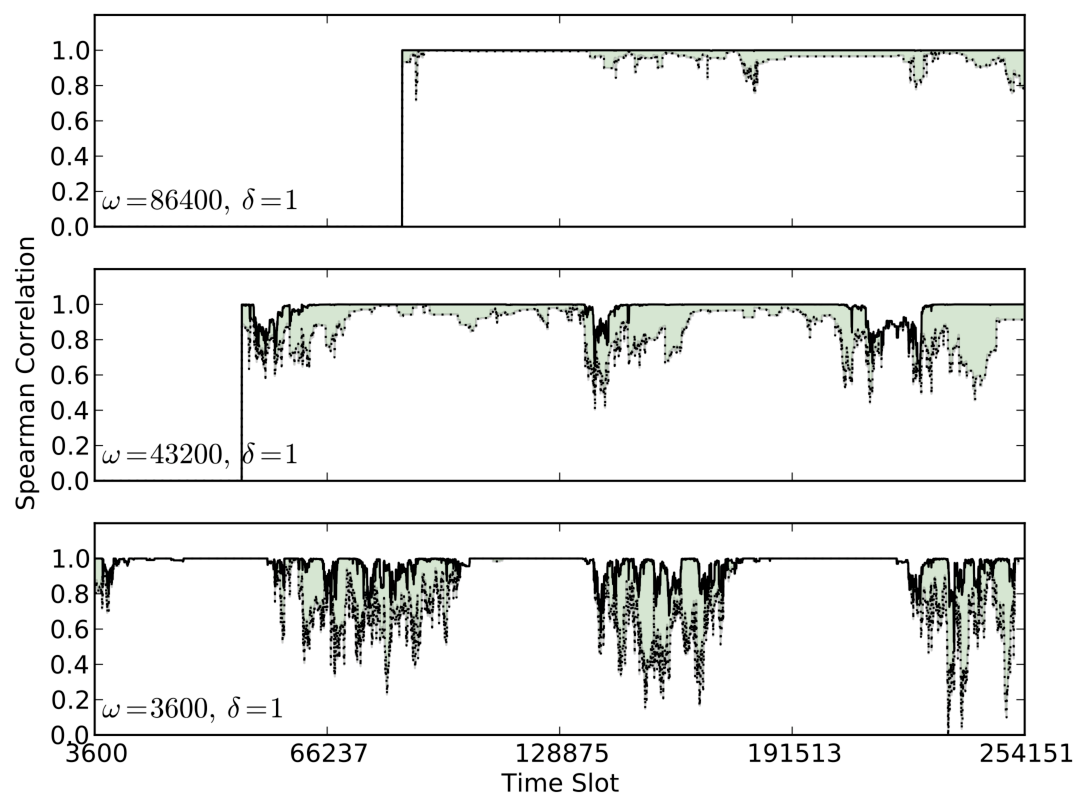
\includegraphics[width=0.49\linewidth, trim=0cm 0cm 0cm 0cm]{cor_spearman_time-step-1.pdf}}
\subfigure[{\em Step size $\delta=3600~seconds\,(=1~hour)$}]{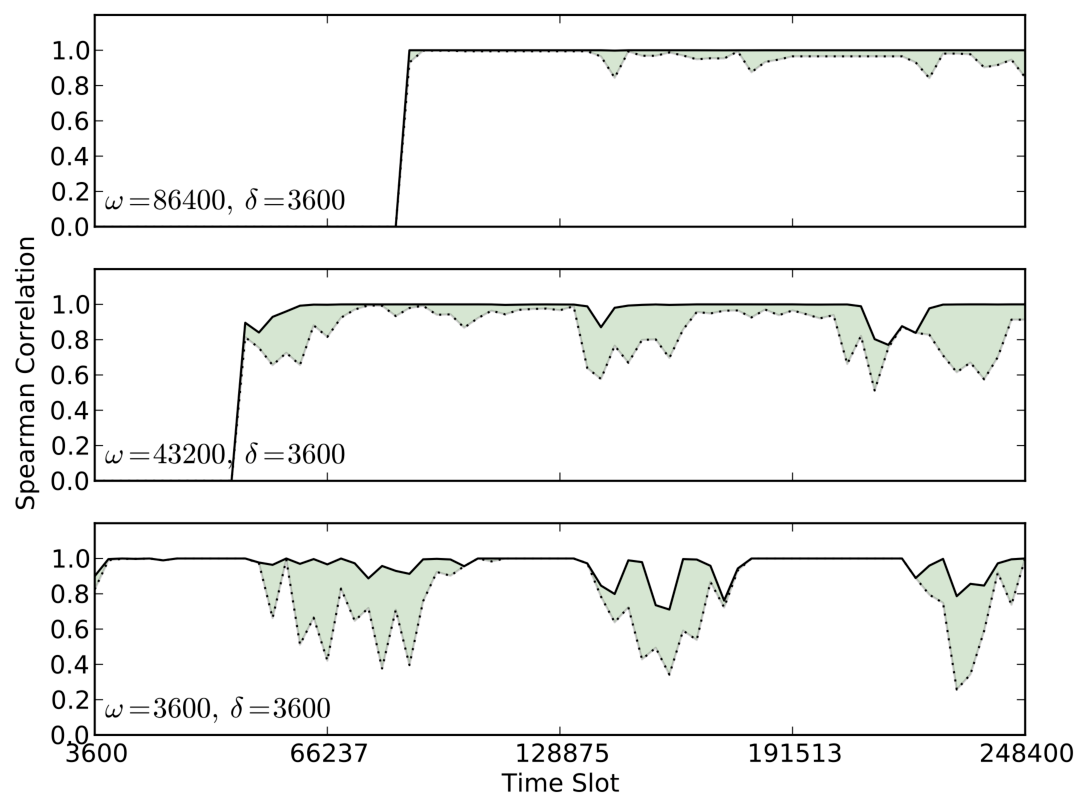
\includegraphics[width=0.49\linewidth, trim=0cm 0cm 0cm 0cm]{cor_spearman_time-step-3600.pdf}}
\caption{Change of correlation between different betweenness metrics over time (the solid line represents the correlation between x-ego betweenness and betweenness whereas the dotted line represents the correlation between ego betweenness and betweenness)}
\label{correlation_gap}
\end{figure*} 
Given a data set, our evaluations identified, for each time window $T_i$, social links between nodes.
In this case, any pair of nodes that communicated with each other for $\theta \cdot \omega / \pi$ time slots or more were assumed to have a social link between them.
On the network consisting of the above nodes and social links, our evaluations then computed the betweenness, ego-betweenness, and x-ego betweenness of each node using the Brandes algorithm~\cite{Brandes01afaster}.
The x-ego betweenness of each node was also computed using our algorithm (Section~\ref{computation}) to experimentally verify the benefit of that algorithm over the Brandes algorithm.

% ///////////////////////////////////
% 
% [older version]
% 
% For all data sets, we convert the original trace data into discrete sequential contact events per unit time per each node pair, and we feed them into each DTN node implemented in our simulation. 
% In a DTN node, the time is discretely slotted in unit of $1$ second from the start time $t_s (=0)$ until the end time $t_e (=\pi)$. For example, $\pi=254,151$ for the {\em Infocom05} data set. 
% %Each node maintains its own clock time, but shares the same length of time slot.\footnote{In real implement, time synchronization over all nodes is not required strictly, but a sophisticated synchronization scheme may help construct more precise ego or x-ego network.} 
% 
% Assuming that each contact lasts one time slot (i.e., each contact starts and ends during the same time slot), {\em a contact between two nodes $v$ and $k$ at time $t_o$} is defined as a 3-tuple $\langle v, k, t_o\rangle$ in our evaluations.\footnote{In spite of asymmetric communication characteristics in general, we assume that reception of a message guarantees a bidirectional contact for the sake of simplicity, like other studies \cite{human_mobility,SIMBET,IEEE:bubble} based on nodes' social behavior.} 
% DTN nodes aggregate its contacts during a {\em time window}, a set of contiguous time slots. 
% The time window size $\omega$ is constant in our simulation and empirically determined in real implement. 
% When time goes by, the time window slides by $\delta$ time slots (i.e., $\delta$ is also called as step size). 
% %If $\delta$ is small, a node will accurately construct its social networks according to its contact behavior, but high computational load will be imposed on each node. Since a node will configure its ego or x-ego network based on contact information in a time window, the social networks will become outdated if the value of $\delta$ is large, but each node can save its CPU cycles. 
% If $\delta$ is small, a node constructs its social networks accurately according to its contact behavior. On the other hand, social networks tend to be outdated if the value of $\delta$ is large.
% Let $T_{0}, T_{1}, \ldots$ denote the ordered sequence of time windows maintained by a node and the $i$th time window $T_{i}$ is defined as follows: $T_i=\{t_{\delta \cdot i}, t_{\delta \cdot i + 1}, t_{\delta \cdot i + 2}, \cdots, t_{\delta \cdot i + \omega - 1}\}$ where $0 \leq i \leq \lfloor\frac{\pi - \omega + 1}{\delta}\rfloor$.
% 
% For a time window $T_i$, a node $v$ maintains its contact duration time $d_{i,k}$ for each node $k$ which $v$ makes a contact during $T_i$. By the definition of contact, $d_{i,k}$ is the number of contacts $\langle v, k, t_o\rangle$ where $t_{\delta \cdot i} \leq t_o \leq t_{\delta \cdot i+\omega-1}$ and it is used to determine its {\em social neighbor nodes} for $T_i$. A node has a predefined threshold $\theta\cdot\omega/\pi$ and sorts out the social neighbor nodes $k'$ where $d_{i,k'} > \theta\cdot\omega/\pi$ at the every end of $T_i$. As explained previously, $\theta$ is pre-determined as a value given by Table \ref{data_set}. For a time window $T_i$, we will denote {\em a set of identifiers of social neighbor nodes} by $N_{v,i}$. 
% 
% %In SimBetTS \cite{SIMBET}, a well-known DTN forwarding scheme based on social graphs, a social link between two nodes is created if there has been at least any contact between them at any time in the past. That is, there is a single time window and $\omega$ is the whole duration of network operation (i.e., $\omega=\pi$). It means that SimBetTS does not consider the time window strategy and the constructed social graphs may get meshed since the whole network operation time contributes to the link creation. Another well-known social network based DTN routing, BUBBLE Rap \cite{IEEE:bubble}, used the similar time window as $T_i$ defined by this section. In the simulation of BUBBLE Rap, both of $\omega$ and $\delta$ were set to the number of time slots corresponding to $6~hours$. It means that two nodes may compare their centrality by using social metrics computed in relatively old time (i.e., $6~hours$ ago). In the two DTN routing schemes, the authors did not consider the quality of social graph fully. In this paper, we vary the values of $\omega$ and $\delta$ so that the diverse social graphs can be evaluated to prove the contribution of this paper. 
% 
% %In the whole simulation time, a DTN node sends {\em Hello} broadcast message periodically with interval of $\tau$ time slots. Each Hello message contains the following information: 1) {\em its own identifier} and 2) {\em a set of identifiers of social neighbor nodes}, the latter of which will be needed by a DTN node to construct its ego or x-ego network. In our simulation, we set $\tau$ to one.
% %During evaluation time, a DTN node sends {\em Hello} broadcast message including its own identifier periodically with interval of $\tau$ time slots. 
% %In our evaluation, we set $\tau$ to one.
% %Since an ego or x-ego network is constructed based on the information about such social neighbor nodes, a node should piggyback $N_{v,i}$ determined at the every end of $T_i$ into the broadcast messages sent during $T_{i+1}$. 
% For each node $k$ which $v$ makes a contact during $T_{i+1}$, $N_{k,i}$ determined at the end of $T_i$ is piggybacked into the contacts $\langle v, k, t_o'\rangle$ made during $T_{i+1}$ where $t_{\delta \cdot (i+1)} \leq t_o' \leq t_{\delta \cdot (i+1)+\omega-1}$ and it is used to configure $v$'s ego and x-ego networks during $T_{i+1}$.
% Since the social neighbor nodes are determined during the previous time window, information in $N_{v,i}$ will be more fresh if the step size $\delta$ of time window is small. At every end of time window $T_i$, $v$ also builds the array $N$ (an input parameter of Algorithm \ref{alg:main}) from $N_{v,i}$ and executes the proposed algorithm. The global network to be compared with ego or x-ego network is also constructed every end of time window $T_i$ by combining all the vertices and edges corresponding to $N_{v,i}$ created by all nodes.    
% 
% ///////////////////////////////////

\subsection{Accuracy of X-Ego Betweenness}\label{accuracy}
\begin{figure*}[t] 
\centering 
\subfigure[{\em Infocom05}]{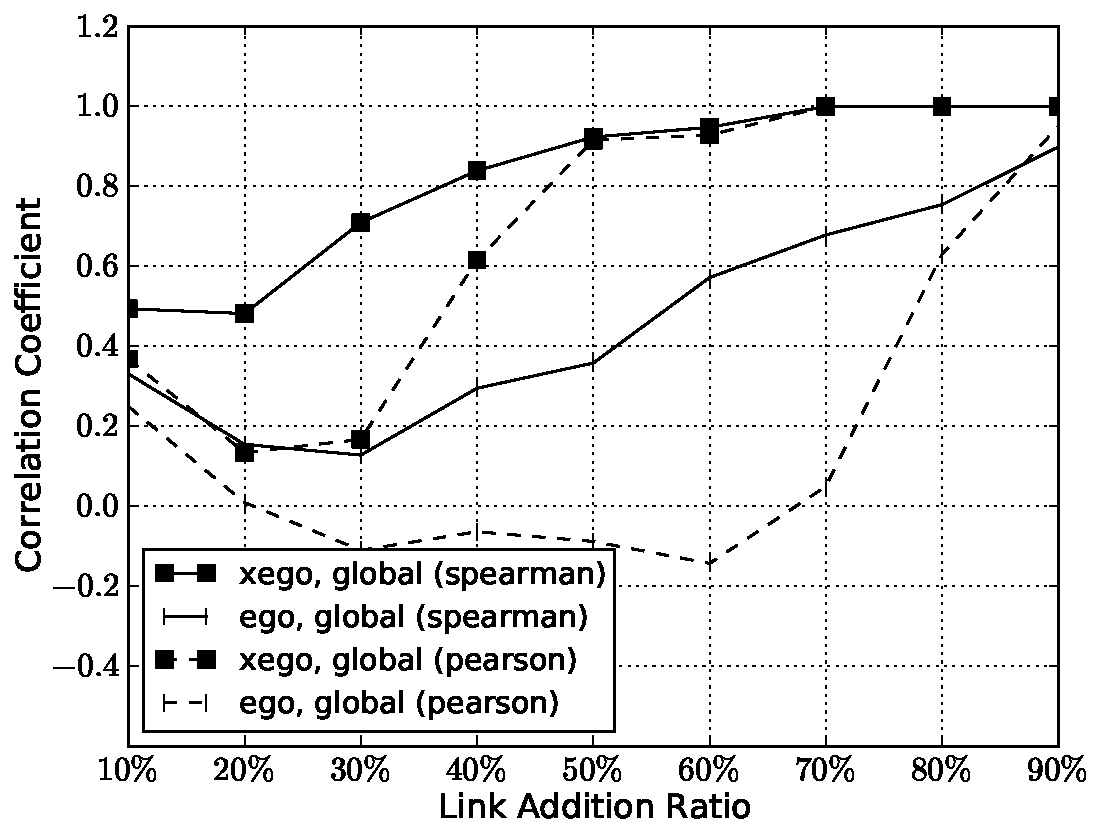
\includegraphics[width=0.246\linewidth, trim=0cm 0cm 0cm 0cm]{1_correlation.pdf}}
\subfigure[{\em Infocom06}]{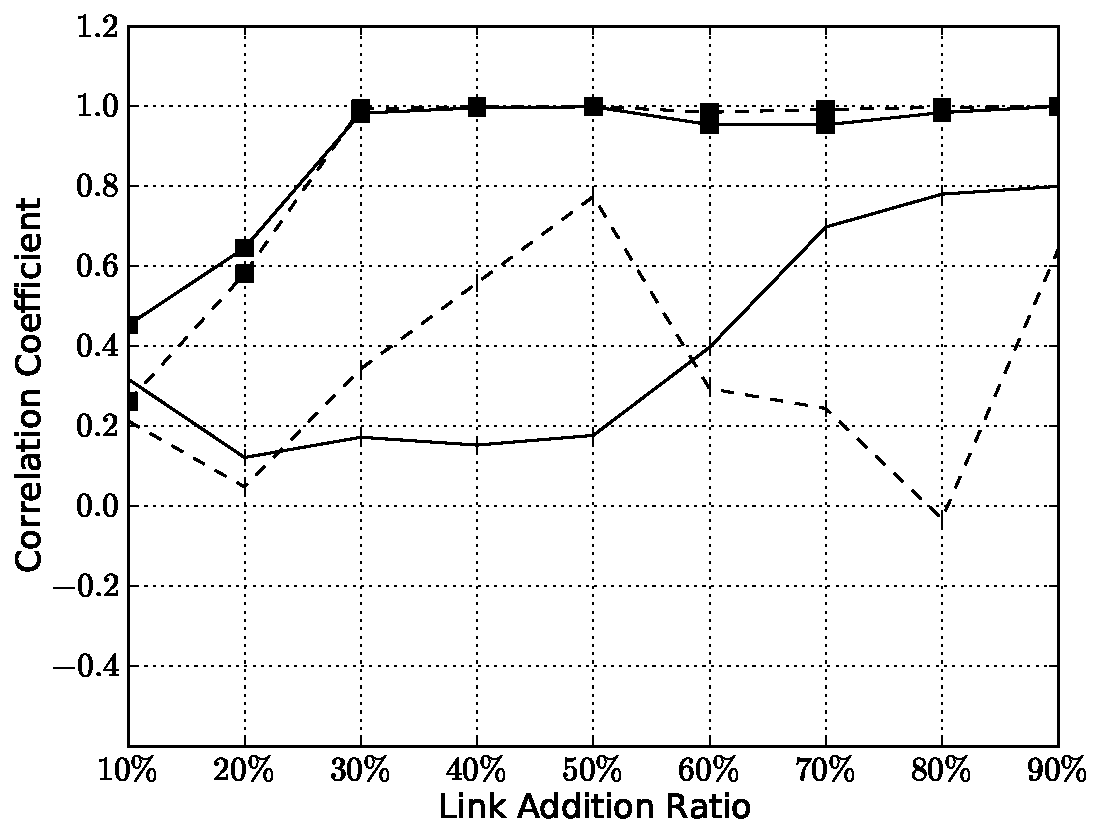
\includegraphics[width=0.246\linewidth, trim=0cm 0cm 0cm 0cm]{2_correlation.pdf}}
\subfigure[{\em Cambridge}]{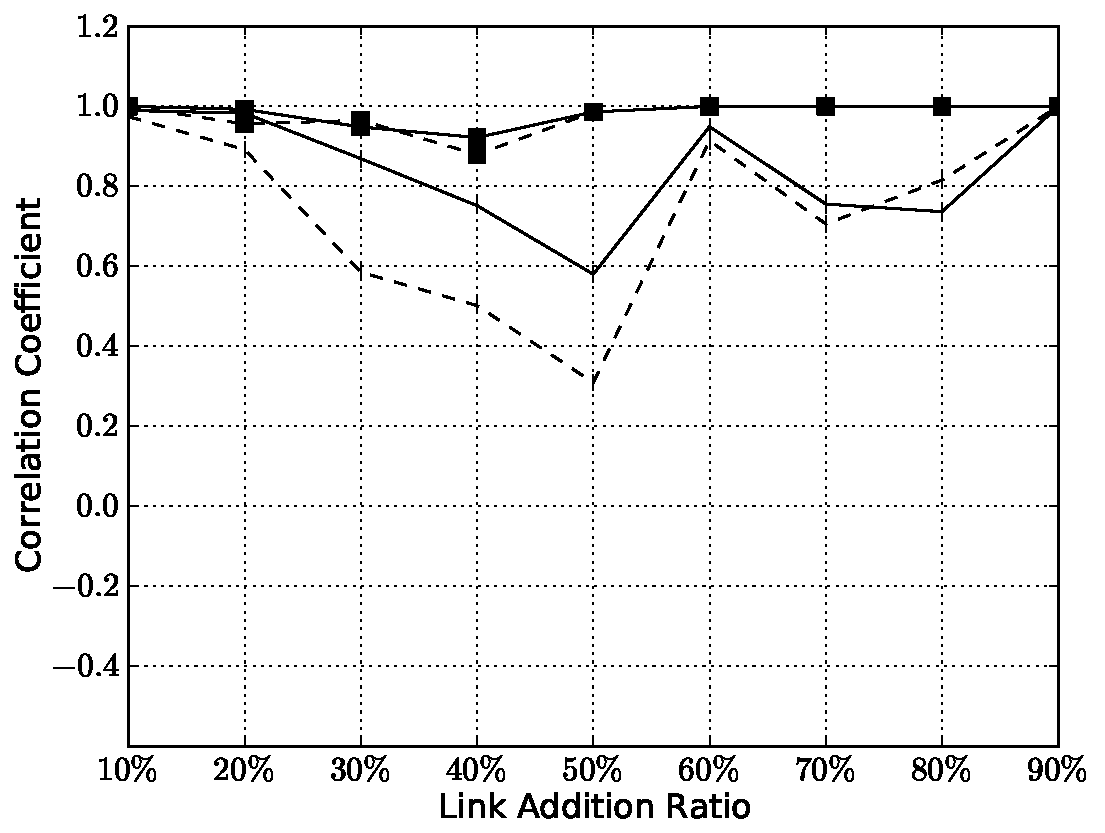
\includegraphics[width=0.246\linewidth, trim=0cm 0cm 0cm 0cm]{3_correlation.pdf}}
\subfigure[{\em Intel}]{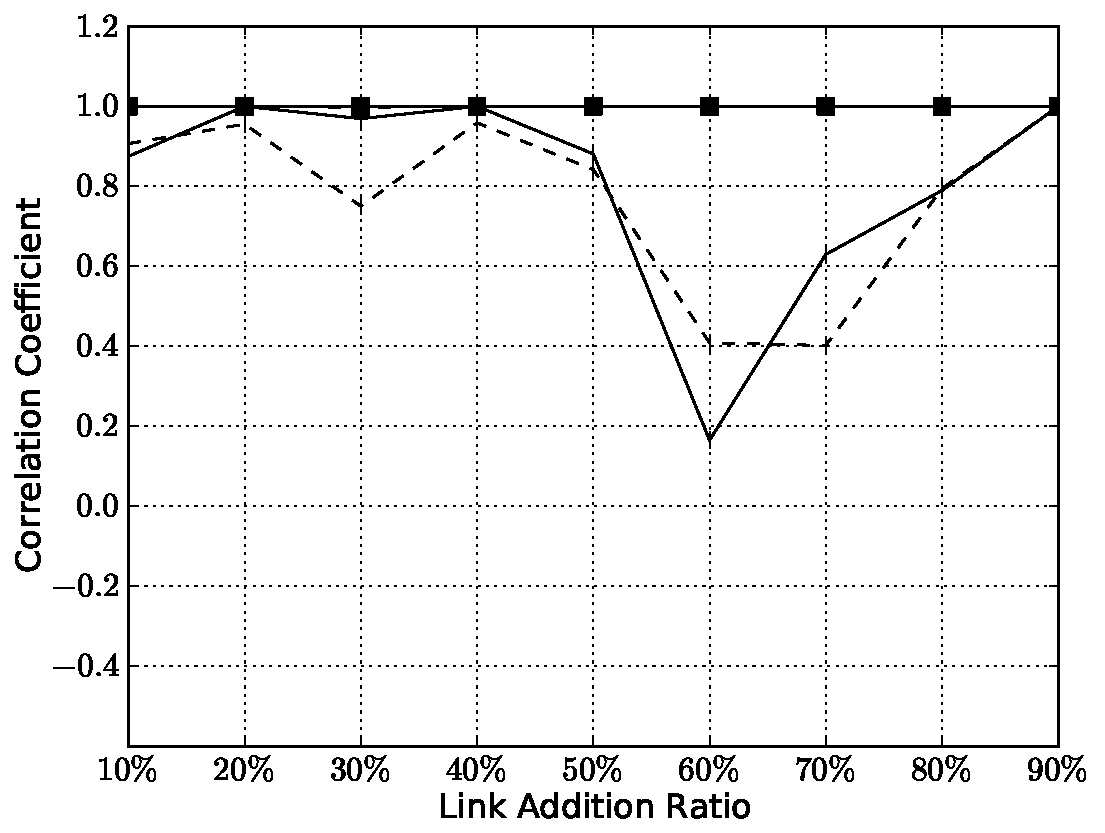
\includegraphics[width=0.246\linewidth, trim=0cm 0cm 0cm 0cm]{4_correlation.pdf}}
\caption{Correlation between different betweenness metrics ($\omega=\pi$)}
\label{correlation_comp}
\end{figure*} 

\begin{figure*}[t]
\centering 
\subfigure[{\em Infocom05}]{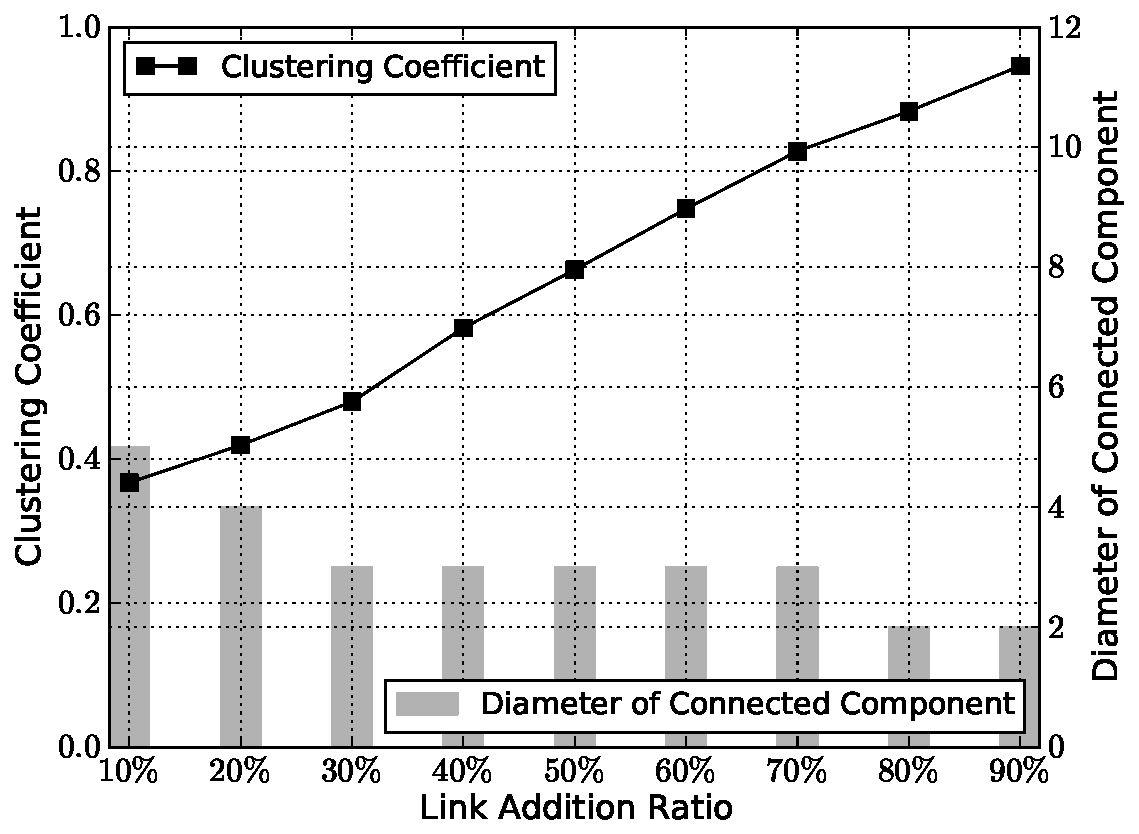
\includegraphics[width=0.246\linewidth, trim=0cm 0cm 0cm 0cm]{1_clustering_and_diameter.pdf}}
\subfigure[{\em Infocom06}]{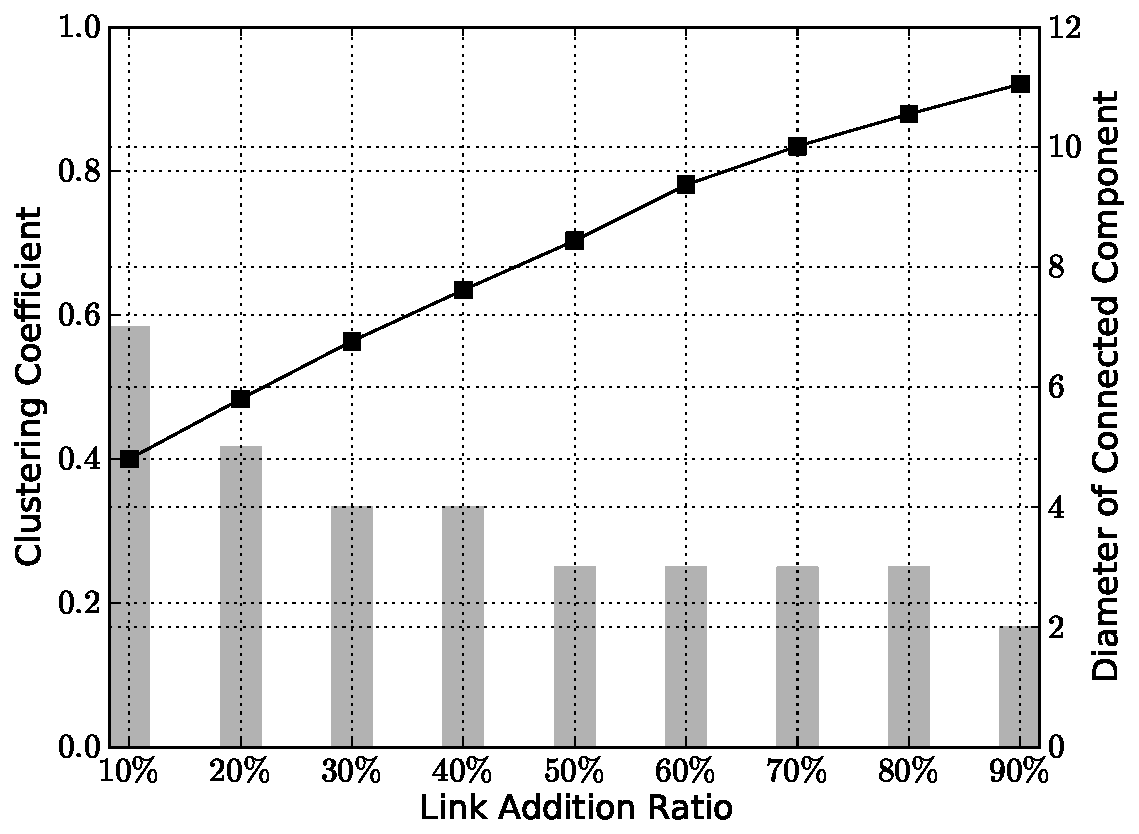
\includegraphics[width=0.246\linewidth, trim=0cm 0cm 0cm 0cm]{2_clustering_and_diameter.pdf}}
\subfigure[{\em Cambridge}]{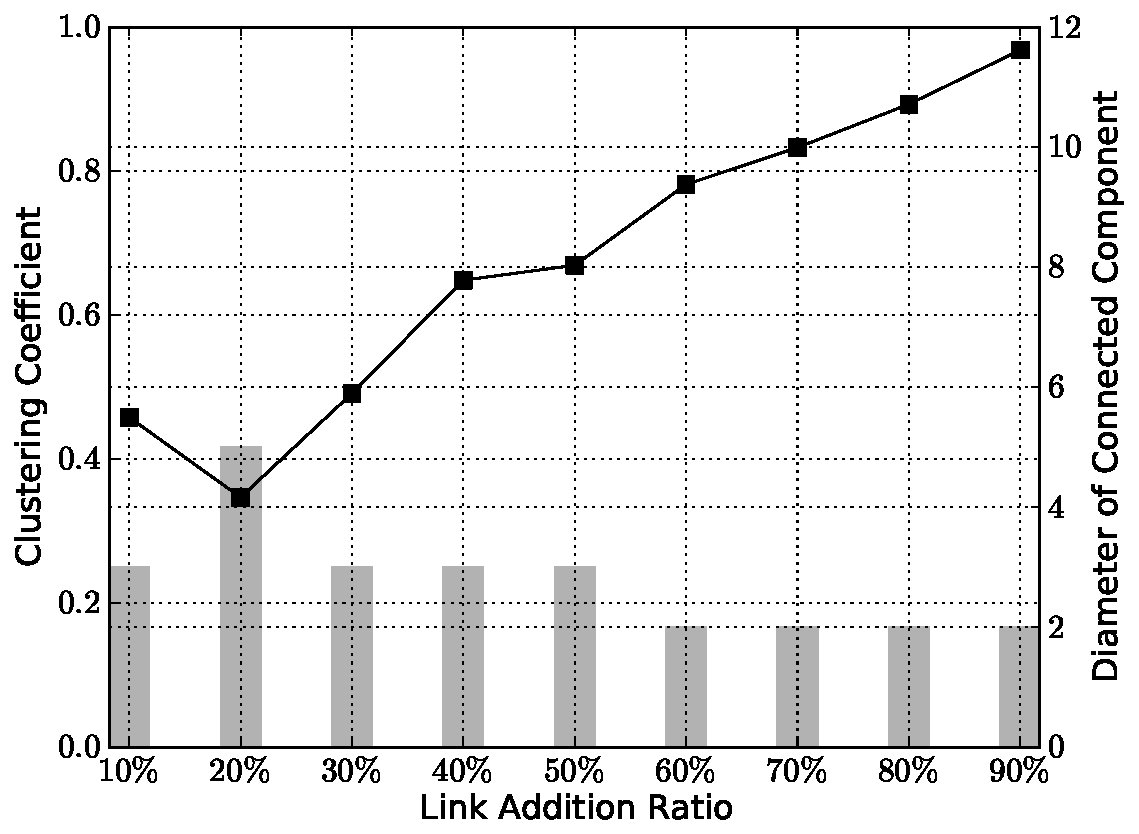
\includegraphics[width=0.246\linewidth, trim=0cm 0cm 0cm 0cm]{3_clustering_and_diameter.pdf}}
\subfigure[{\em Intel}]{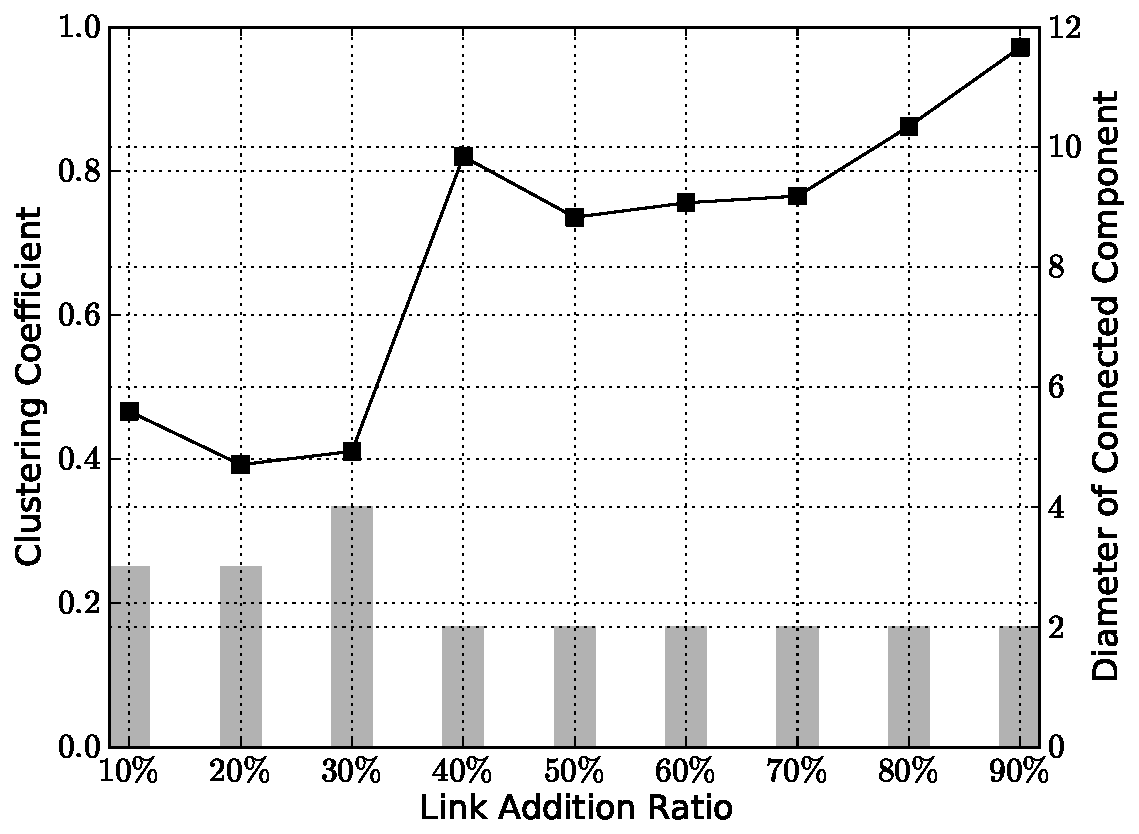
\includegraphics[width=0.246\linewidth, trim=0cm 0cm 0cm 0cm]{4_clustering_and_diameter.pdf}}
\caption{Clustering coefficient and diameter of  connected component ($\omega=\pi$)}
\label{netinfo1}
\end{figure*} 

\begin{figure*}[t] 
\centering 
\subfigure[{\em Infocom05}]{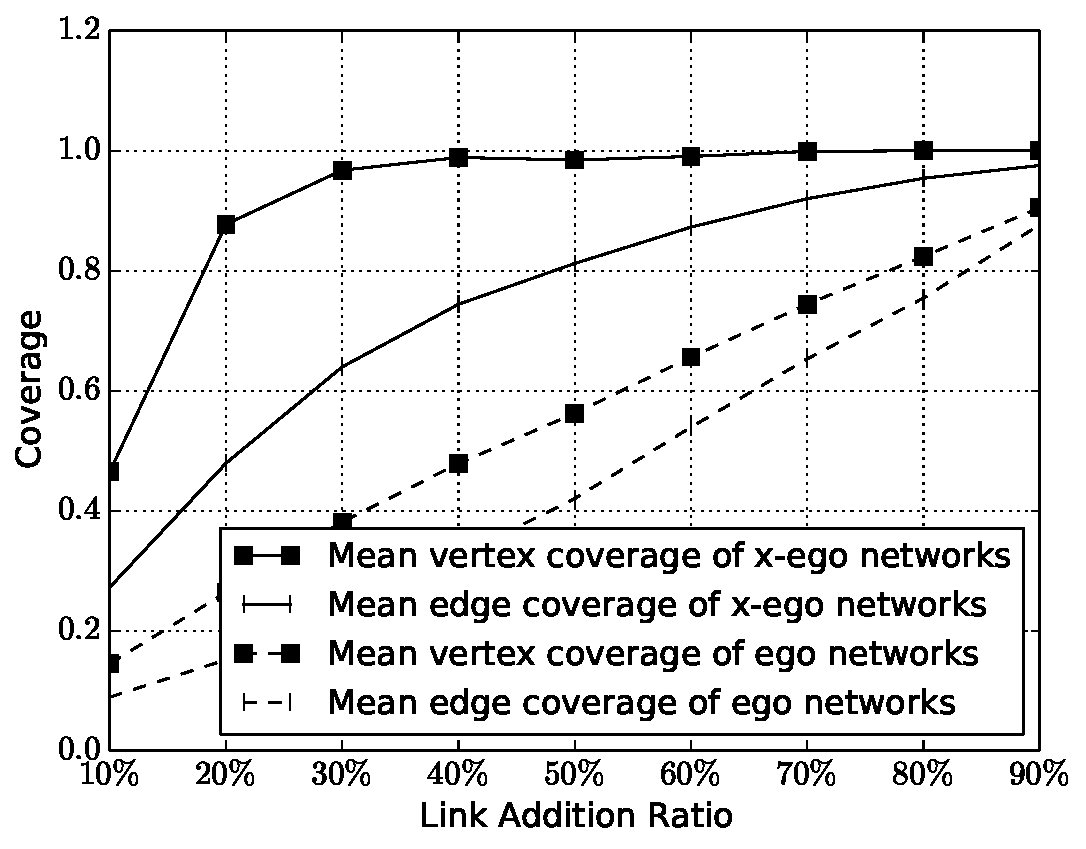
\includegraphics[width=0.246\linewidth, trim=0cm 0cm 0cm 0cm]{1_graph_info_2.pdf}}
\subfigure[{\em Infocom06}]{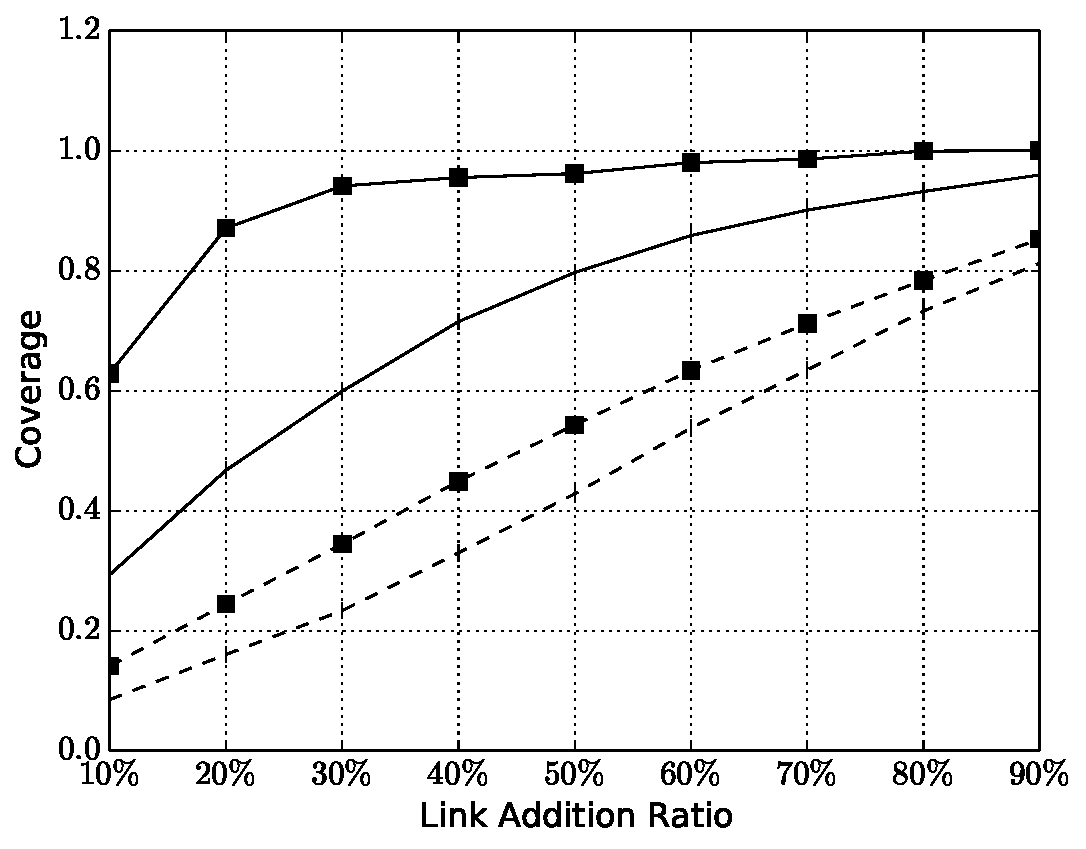
\includegraphics[width=0.246\linewidth, trim=0cm 0cm 0cm 0cm]{2_graph_info_2.pdf}}
\subfigure[{\em Cambridge}]{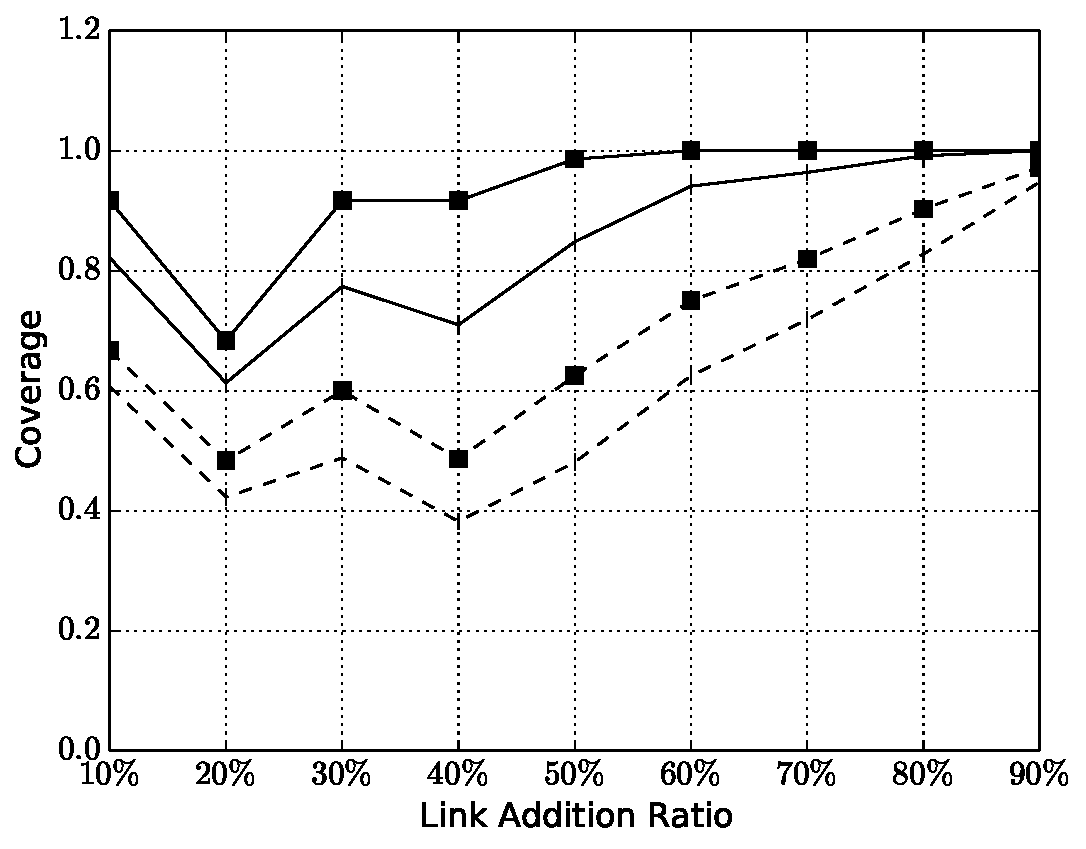
\includegraphics[width=0.246\linewidth, trim=0cm 0cm 0cm 0cm]{3_graph_info_2.pdf}}
\subfigure[{\em Intel}]{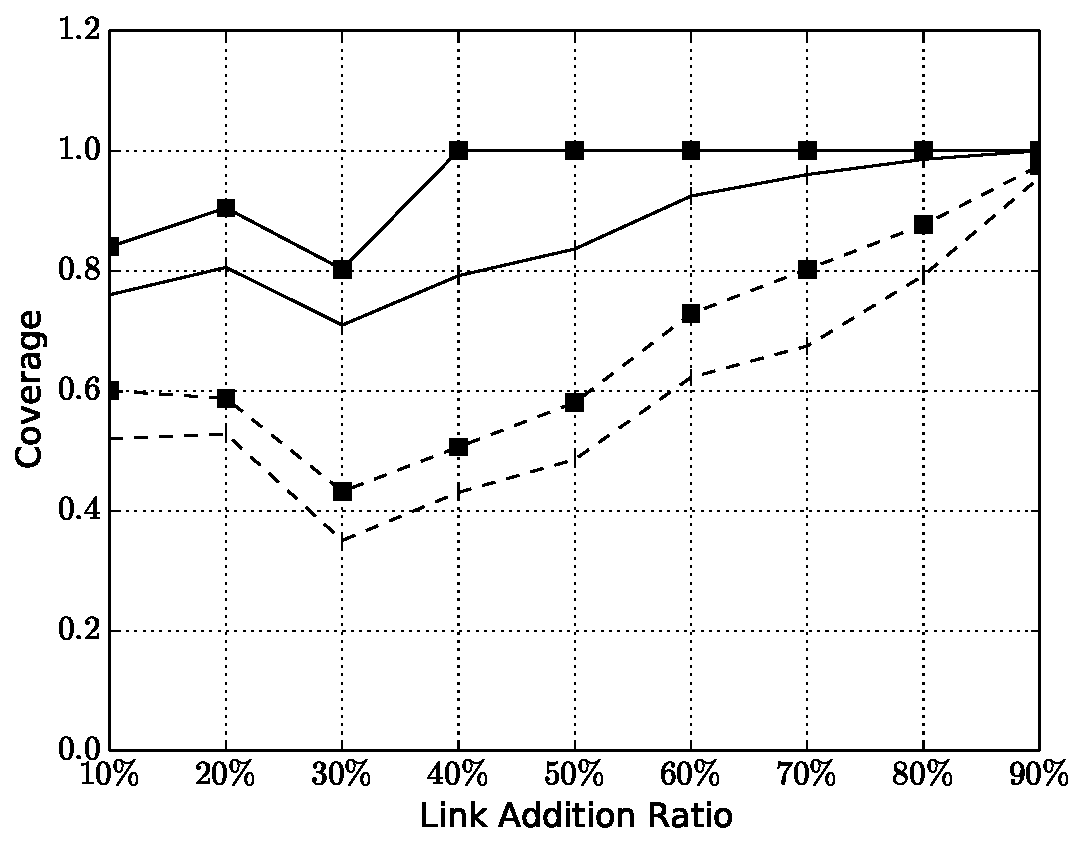
\includegraphics[width=0.246\linewidth, trim=0cm 0cm 0cm 0cm]{4_graph_info_2.pdf}}
\caption{Coverage of x-ego and ego networks over the global network ($\omega=\pi$)}    
\label{netinfo2}
\end{figure*}
%, $\NX$ and $\MX$: the average number of vertices and edges in x-ego networks, $\NE$ and $\ME$: the average number of vertices and edges in ego networks, $\NC$ and $\MC$: the average number of vertices and edges in connected components when, for each node, the connected component containing that node is considered
% Fig.~\ref{correlation_gap} shows the variation of gap between the Spearman correlation between $\BX{v}$ and $\B{v}$ and the one between $\BE{v}$ and $\B{v}$ over time slots. 
Fig.~\ref{correlation_gap} compares the accuracy of x-ego betweenness and ego betweenness in terms of their similarity to betweenness.
Each subfigure in Fig.~\ref{correlation_gap} shows the variation of the Spearman correlation between x-ego betweenness and betweenness (the dotted line) and that between ego betweenness and betweenness (the solid line).
% The data set {\em Infocom05} is used with time window size $\omega$ set to $86,400\,sec.\,(=24\,hours)$, $43,200\,sec.\,(=12\,hours)$ or $3,600\,sec.\,(=1\,hour)$, and step size $\delta$ set to $1\,sec.$ or $3,600\,sec$. 
The results illustrated in the figures were obtained from the {\em Infocom05} data set with the time window size $\omega$ set to 24 hours (86,400 seconds), 12 hours (43,200 seconds), or 1 hour (3,600 seconds) and the step size $\delta$ set to 1 second or 3,600 seconds.
% Edge creation ratio is $50\%$ so that a DTN node makes a social link with other node if the accumulated contact duration time is more than $1,609\cdot86,400/3,600\, (=38,616\,sec.)$ when $\omega=86,400$ and $\delta=3,600$. 
Furthermore, the link addition ratio was set to $50\%$ (equivalently, the contact duration threshold was set to 1,609 seconds).
For this reason, when $\omega=86{,}400$ and $\delta=3{,}600$, a node assumed a social link with another node if the accumulated contact duration between these nodes was longer than $1{,}609 \cdot 86{,}400 / 254{,}151\, (=546.9)$ seconds. 
% In each figure, there are two lines, each of which represents the spearman correlation between $\BX{v}$ and $\B{v}$, and between $\BE{v}$ and $\B{v}$, respectively. 
% We fill the space between the two lines to make the gap between them obvious. 

% It is observed in the figure that $\BX{v}$ is more correlated to $\B{v}$ than $\BE{v}$, which also means $\BX{v}$ is more accurate than $\BE{v}$.
Fig.~\ref{correlation_gap} shows that x-ego betweenness is more strongly correlated to betweenness than ego betweenness (i.e., x-ego betweenness is more accurate than ego betweenness) across different time window sizes and step sizes.
As the window step size ($\delta$) increases from 1 second (Fig.~\ref{correlation_gap} (a)) to 3,600 seconds (Fig.~\ref{correlation_gap} (b)), the betweenness of each vertex is computed/updated less frequently, thereby saving communication and computation resources at the expense of timeliness of betweenness values. 
% We can also know that both correlation values become very high when the time window size gets long. 
% It is because a DTN node can determine its local centrality more accurately if it uses sufficient information in a large window size. 
When the window step size ($\delta$) is fixed, as the time window size ($\omega$) increases, the variation of correlation between x-ego betweenness and betweenness decreases since the overlap between consecutive windows increases.
Given a larger time window, the correlation between x-ego betweenness and betweenness also increases since the x-ego network of each node may include more nodes (i.e., the accuracy of x-ego betweenness may improve).
% It also shows higher correlation values as the time window size ($\omega$) increases.
% In addition to that, the values are invariable since sliding step is not much high in comparison with the time window size and the past contact information is still used to get the values. 
%On the other hand, the correlation values become low and variable when the time window size gets short. 
% Even though the time window size is short, however, the correlation between $\BX{v}$ and $\B{v}$ is not much low: just $2.8\%$ of correlation values between $\BX{v}$ and $\B{v}$ over time slots is less than 0.8 when $\omega=3600$ and $\delta=1$, and $7.5\%$ when $\omega=3600$ and $\delta=3600$. 
On the other hand, even with small time windows, the overall correlation between x-go betweenness and betweenness remains high. 
For example, in Fig.~\ref{correlation_gap}, only $2.8\%$ of correlation values between x-ego betweenness and betweenness are smaller than 0.8 when $\omega=3{,}600$ and $\delta=1$, and only $7.5\%$ when $\omega=3{,}600$ and $\delta=3{,}600$. 

% Fig.~\ref{correlation_comp} shows the Spearman and Pearson correlation variation over diverse edge creation ratio and data sets. 
Fig.~\ref{correlation_comp} shows the correlation between x-ego betweenness and betweenness as well as between ego betweenness and betweenness across diverse link addition ratios and data sets.
% In this evaluation, all contact information over simulation duration are included into only one time window (i.e., $\omega = 2.9, 3.9, 5.3$ and $4.2$ days for each data set, respectively). 
This result was obtained by considering all contact information from each data set using a time window that corresponds to the data collection period (i.e., $\omega = 2.9, 3.9, 5.3$ and $4.2$ days for {\em Infocom05}, {\em Infocom06},  {\it Cambridge} and {\it Intel}, respectively).
% For the edge creation ratio/threshold values, we used the same values as the ones shown in Table \ref{data_set}. 
For each combination of data set and link addition ratio, we used the contact duration threshold shown in Table \ref{data_set}. 
% From the evaluation results, we found the followings: 
% \begin{itemize}
%   \item[1)] $\BX{v}$ is more highly correlated to globally computed betweenness $\B{v}$ than $\BE{v}$.
%   \item[2)] The correlation value between $\BX{v}$ and $\B{v}$ is very high (almost one) in most cases and it is even always one when small number of nodes constitute the DTN network like {\em Cambridge} or {\em Intel}.
% \end{itemize}

Fig.~\ref{correlation_comp} illustrates that:
\begin{itemize}
  \item[1)] X-ego betweenness is more strongly correlated to betweenness than ego betweenness (i.e., x-ego betweenness is more accurate than ego betweenness).
  \item[2)] The correlation between x-ego betweenness and betweenness is almost one in most cases. 
Furthermore, in the cases of {\em Cambridge} and {\em Intel}, where a small number of nodes constitute a network, the correlation between x-ego betweenness and betweenness is very close to one across all link addition ratios.
\end{itemize} 
% These features make $\BX{v}$ a proper measure for social-aware DTN routing schemes making use of betweenness centrality as the core metric of forwarding policy, since they are not trying to compare the absolute centrality values of each node but rather to determine which nodes are more central than others. 
% On the other hand, it is observed the Spearman and Pearson correlations between $\BE{v}$ and $\B{v}$ are very low in many cases. 
In contrast to the high correlation between x-ego betweenness and betweenness, the correlation between ego betweenness and betweenness is noticeably low in many cases.
% For example, it is mostly below 0.8 in the all data sets, and also mostly below 0.6 in {\em Infocom05} and {\em Infocom06} data sets, respectively. 
For example, it is mostly below 0.8 for all of the data sets and also mostly below 0.6 for {\em Infocom05} and {\em Infocom06}.
% These results show that the data delivery efficiency could be not high if social-aware DTN forwarding schemes would rely on $\BE{v}$.
The above results indicate the superiority of x-ego betweenness over ego betweenness in wireless networks.


% As shown in Fig. \ref{correlation_comp}, the correlation values become high if more edges are included into ego or x-ego networks (i.e.,  the network becomes dense), while they are mostly very low when the network is sparse. 
% For example, the lowest value of Spearman correlation between $\BX{v}$ and $\B{v}$ is $0.4819$ and $0.4535$ when the edge creation ratio is $20\%$ at the {\em Infocom05} data set and $10\%$ at the {\em Infocom06} data set, respectively. 
% The lowest value in {\em Cambridge} data set are found even when the ratio is relatively high, i.e., $0.4$. 
% In order to understand these results better, we investigate diverse metrics on network structure,  and study the relation between the correlation and them. 
% The results are depicted in Fig. \ref{netinfo1} and \ref{netinfo2}. 
\begin{figure*}[t]
\centering
\subfigure[{\em Infocom05}]{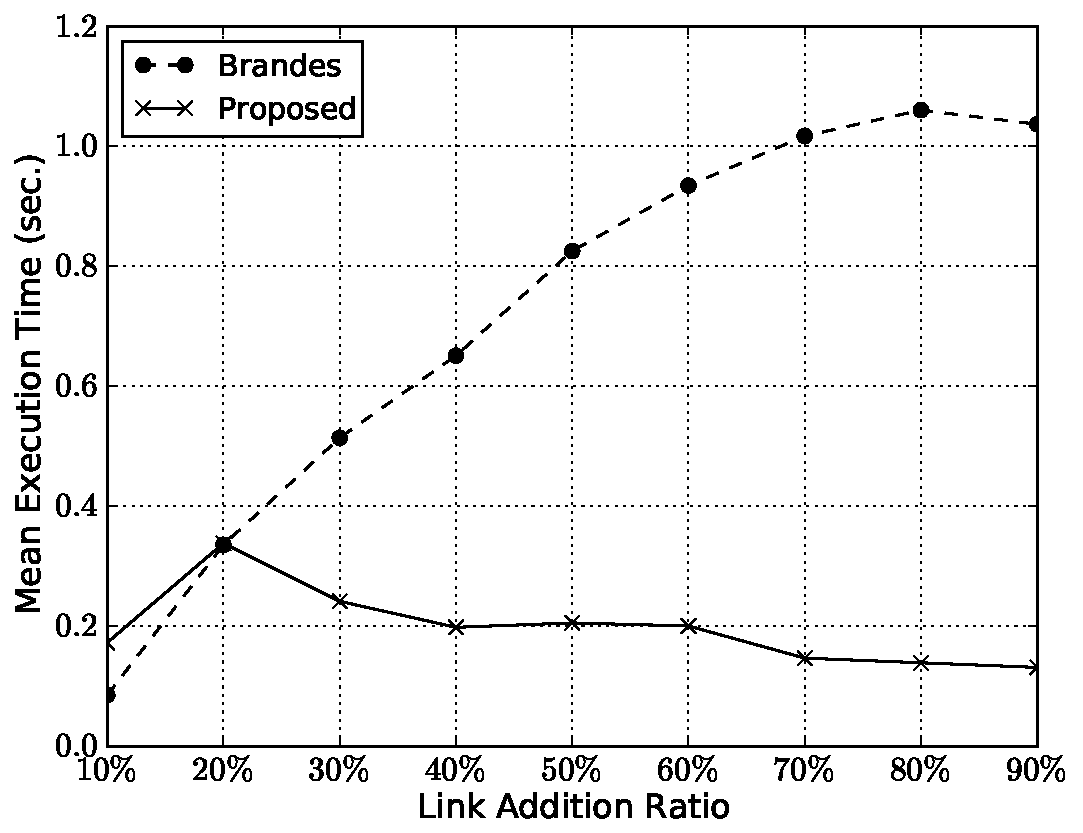
\includegraphics[width=0.24\linewidth, trim=0cm 0cm 0cm 0cm]{1_xEgo_elapsed_time.pdf}}
\subfigure[{\em Infocom06}]{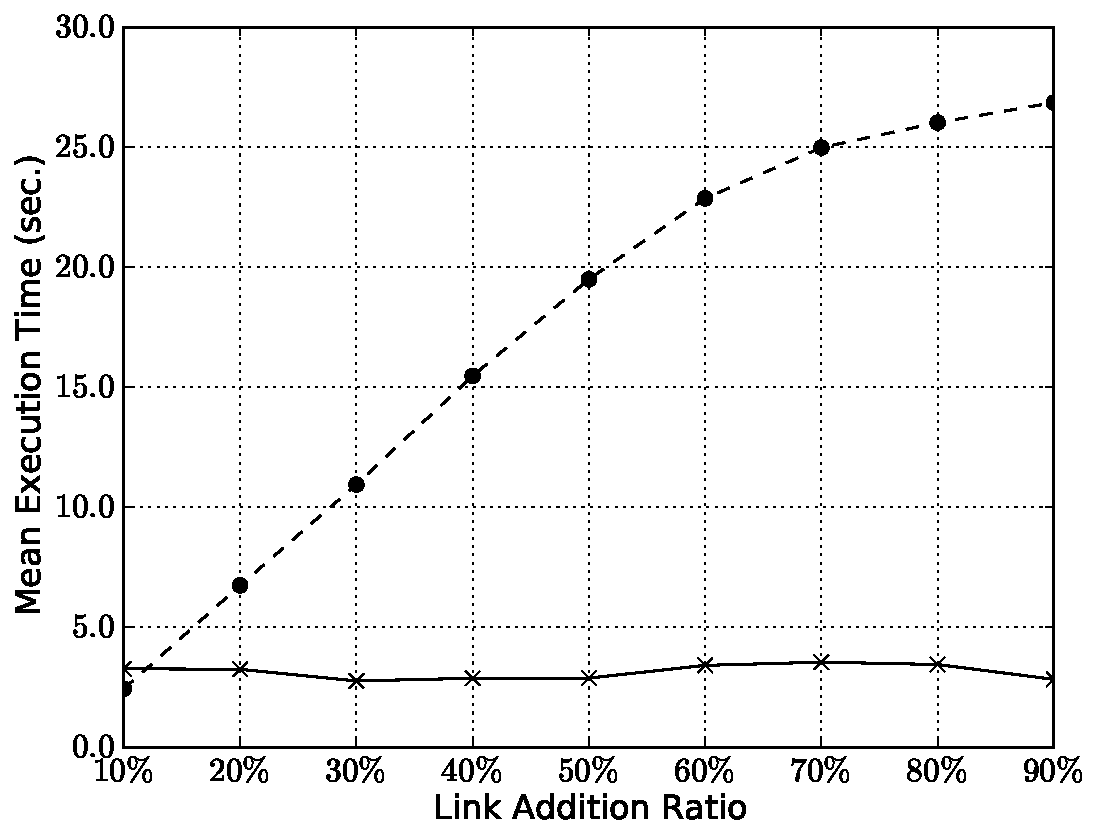
\includegraphics[width=0.243\linewidth, trim=0cm 0cm 0cm 0cm]{2_xEgo_elapsed_time.pdf}}
\subfigure[{\em Cambridge}]{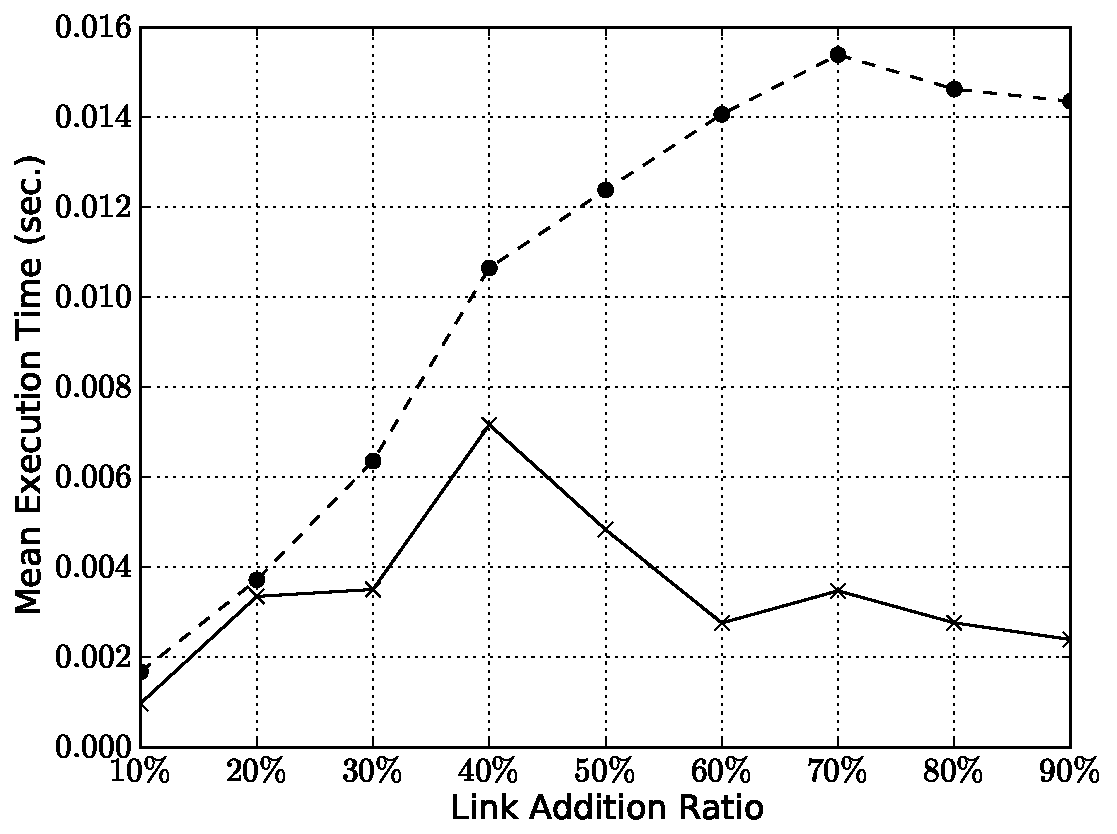
\includegraphics[width=0.247\linewidth, trim=0cm 0cm 0cm 0cm]{3_xEgo_elapsed_time.pdf}}
\subfigure[{\em Intel}]{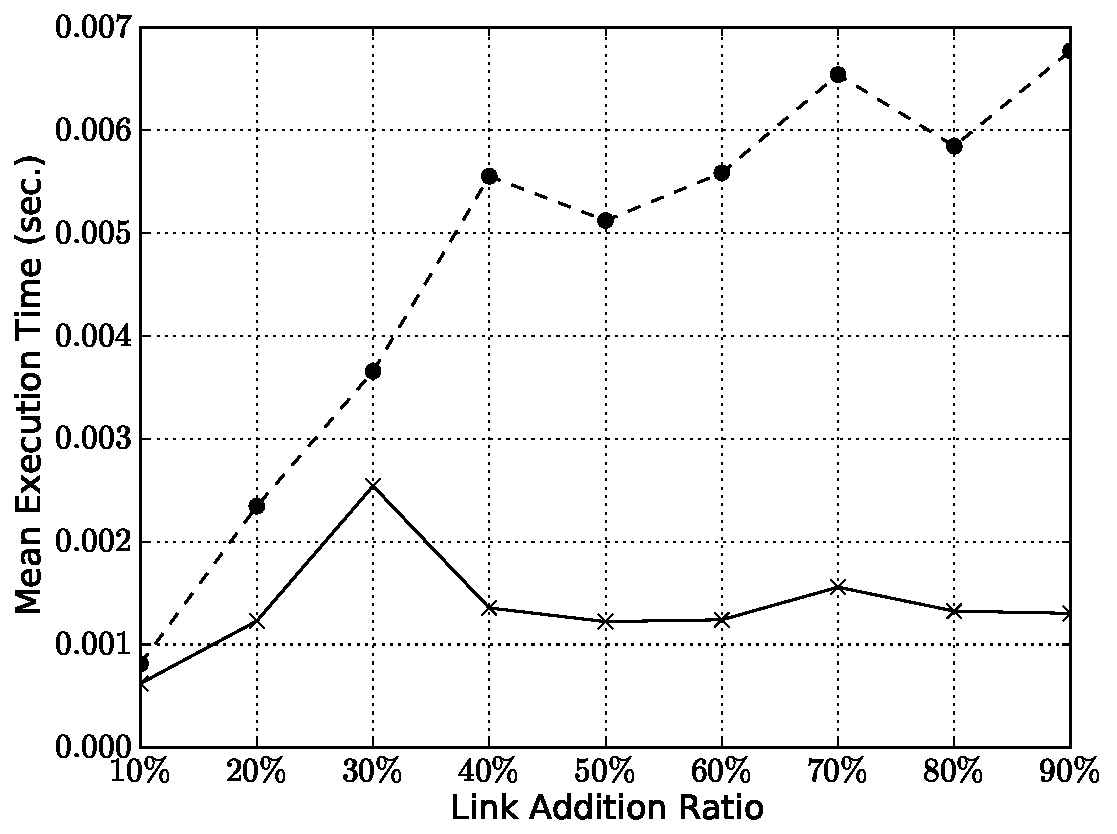
\includegraphics[width=0.247\linewidth, trim=0cm 0cm 0cm 0cm]{4_xEgo_elapsed_time.pdf}}
\caption{Comparison of algorithm execution speed to get x-ego betweenness}
\label{speed}  
\end{figure*}

\begin{figure*}[t]
\centering
\subfigure[{\em Infocom05}]{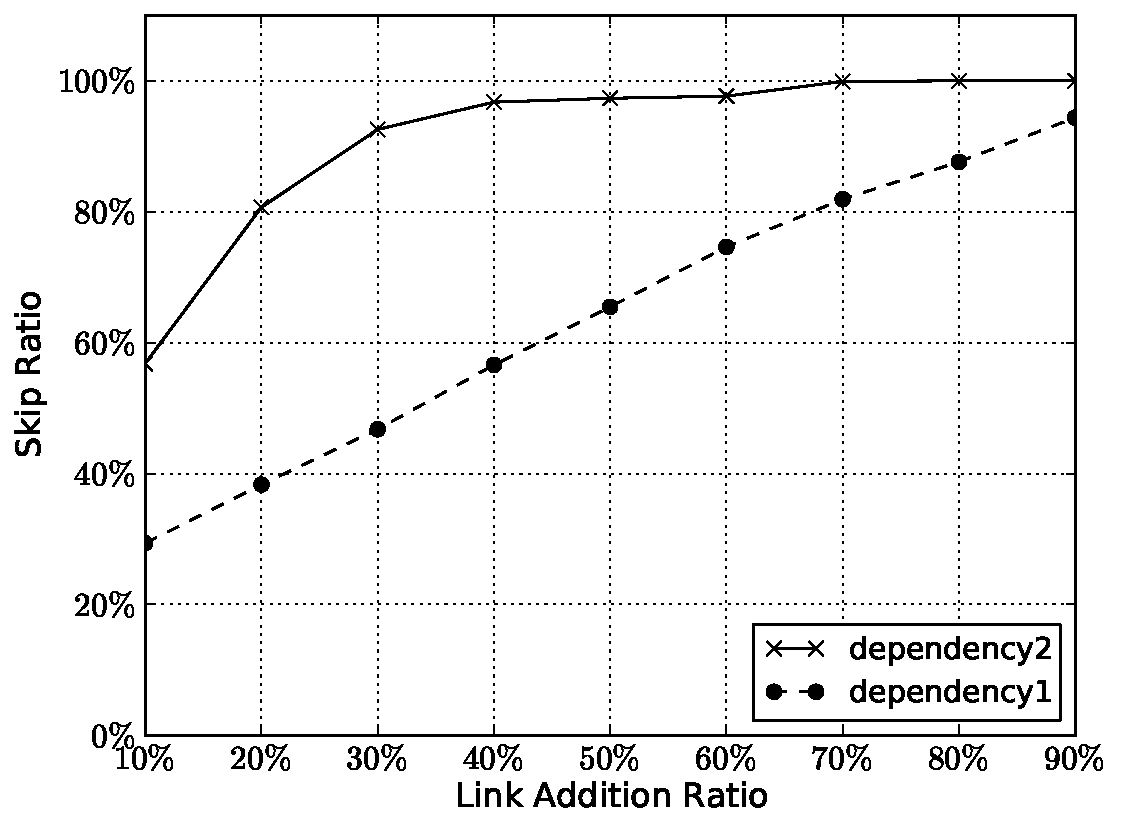
\includegraphics[width=0.246\linewidth, trim=0cm 0cm 0cm 0cm]{1_xEgo_skip_rate.pdf}}
\subfigure[{\em Infocom06}]{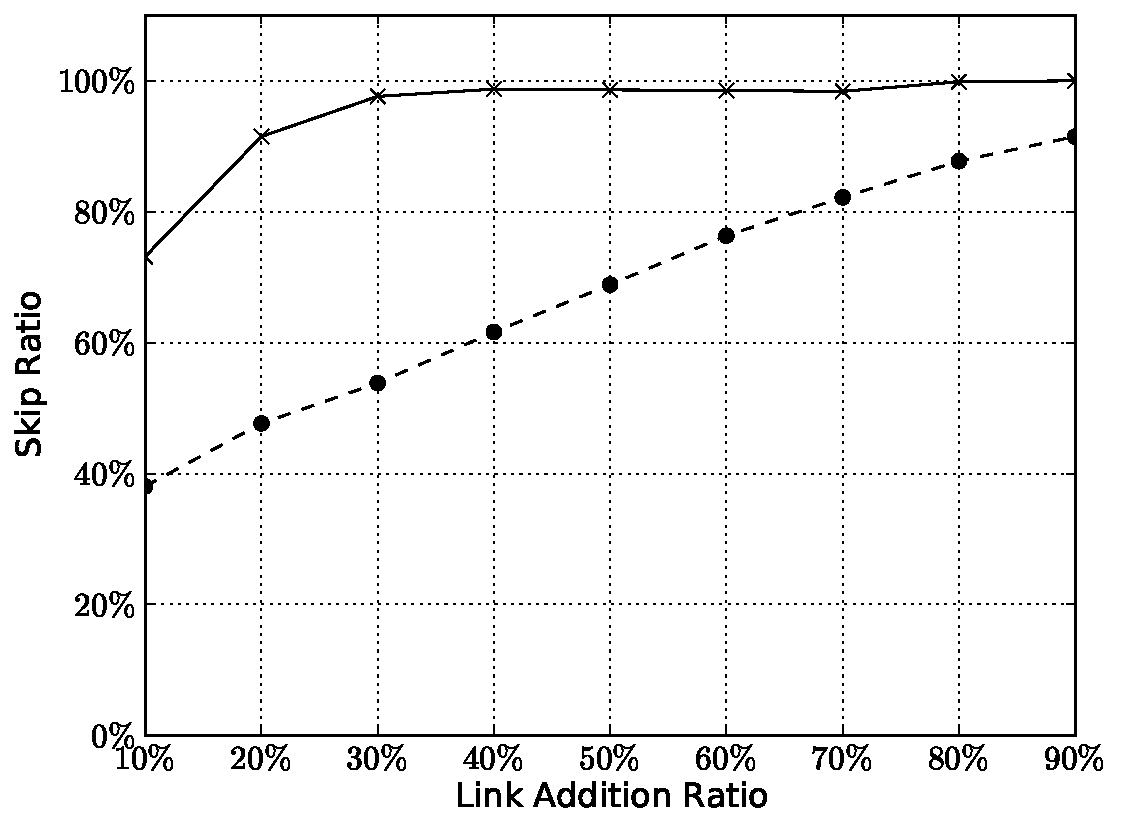
\includegraphics[width=0.246\linewidth, trim=0cm 0cm 0cm 0cm]{2_xEgo_skip_rate.pdf}}
\subfigure[{\em Cambridge}]{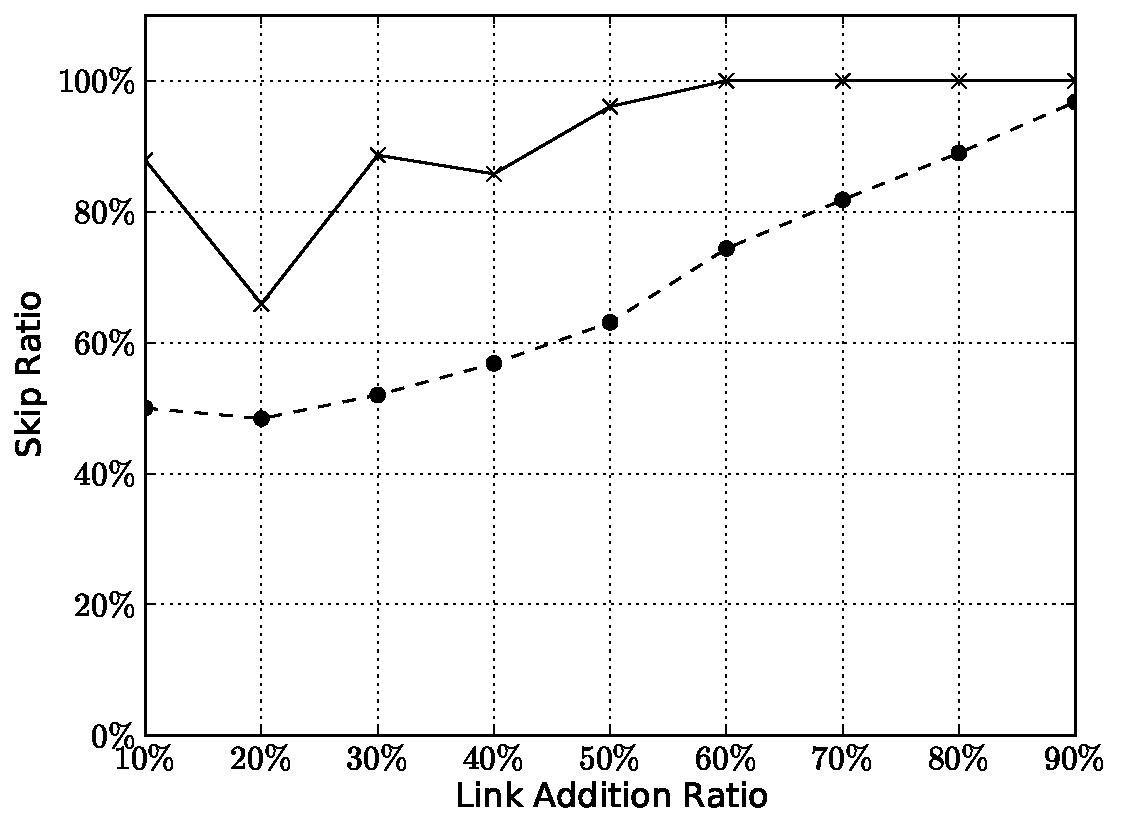
\includegraphics[width=0.246\linewidth, trim=0cm 0cm 0cm 0cm]{3_xEgo_skip_rate.pdf}}
\subfigure[{\em Intel}]{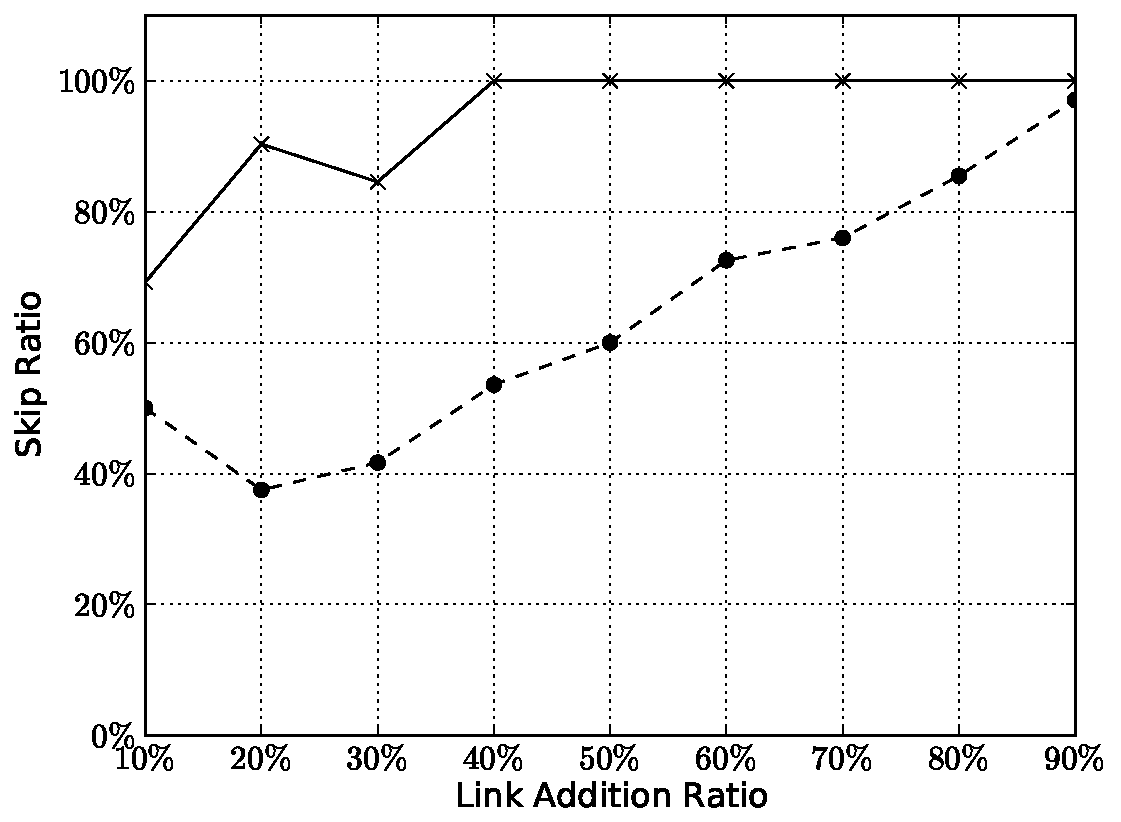
\includegraphics[width=0.246\linewidth, trim=0cm 0cm 0cm 0cm]{4_xEgo_skip_rate.pdf}}
\caption{Skip ratio in the proposed algorithm}
\label{skip}
\end{figure*}
 
In Fig.~\ref{correlation_comp}, while the same network overhead is required for both x-ego betweenness and ego betweenness (Section~\ref{x-ego_definition}), the correlation between x-ego betweenness and betweenness is consistently higher than the correlation between ego betweenness and betweenness. 
There are, however, link addition ratios (e.g., 10\% and 20\% in Fig.~\ref{correlation_comp} (a) and Fig.~\ref{correlation_comp} (b)) that lead to relatively low correlation between x-ego betweenness and betweenness.
To understand these situations, we obtained further evaluation results that are depicted in Fig.~\ref{netinfo1} and Fig.~\ref{netinfo2}. 

% Fig. \ref{netinfo1} shows the clustering coefficient and the diameter of the component in the global networks. When we compare a figure in Figure \ref{netinfo1} with the corresponding figure in Figure \ref{correlation_comp}, we can observe the followings:
% \begin{itemize}
% \item[1)] The correlation values are mostly proportional to the clustering coefficient of global network.
% \item[2)] The correlation values are mostly in inverse proportion to the network diameter of global network.
% \item[3)] The accuracy of $\BX{v}$ tends to be low when the network diameter of global network is more than 4.
% \end{itemize} Among the above findings, the third one is because x-ego networks include only 1 and 2-hop neighbors of a DTN node. Therefore, a DTN nodes need to keep the edge creation ratio more than roughly $30\%$. On the other hand, the above features are not distinct when the scale of network is low. 

Fig.~\ref{netinfo1} shows, for each data set, the impact of link addition ratio on the clustering coefficient and the average diameter of the connected components in the corresponding network.
As more links are added, the 1-hop neighbors of each node tend to have more links between them (i.e., the clustering coefficient increases) and the shortest path length between nodes tends to decrease (i.e., the diameter of the connected component containing the node decreases).\footnote{For the link addition ratio of 10\% in Figure~\ref{netinfo1} (c) and the same of 10\% and 20\% in Figure~\ref{netinfo1} (d), the network diameter is unusually small since, due to a very small number of links in the underlying network, each node has only a few reachable nodes and the latter are within 2 hops away from the former.}
Fig.~\ref{correlation_comp} and Fig.~\ref{netinfo1} show that x-ego betweenness and betweenness are strongly correlated when the average diameter of the connected components is less than 4.
In such cases, there is a large overlap between the x-ego network of a node and the connected component containing that node (i.e., x-betweenness is an accurate estimation of betweenness).
% As shown in Figure \ref{netinfo2}, we also examined two coverage ratios of ego or x-ego network to global network: 1) vertex coverage ($\NX/\NC$ and $\NE/\NC$) and 2) edge coverage ($\MX/\MC$ and $\ME/\MC$). 
% We can observe that x-ego networks cover most vertices in connected components containing the corresponding ego node in the global network, when the edge creation ratio is not low. 
% On the other hand, ego networks do not cover much vertices and edges in the connected components for most cases. 
% These coverage gaps become the fundamental reason that $\BX{v}$ is more highly correlated to globally computed betweenness $\B{v}$ than $\BE{v}$.

%Fig.~\ref{netinfo2} shows the size of x-ego and ego networks compared to the underlying DTN.
Fig.~\ref{netinfo2} shows the size of x-ego and ego networks compared to the global network. 
For this result, we found, for each node $v$, the number of vertices in the x-ego network of $v$ (denoted as $|\XN{v}(V)|$) and that in the ego network of $v$ (denoted as $|\EN{v}(V)|$) as well as the number of edges in the x-ego network of $v$ (denoted as $|\XN{v}(E)|$) and that in the ego network of $v$ (denoted as $|\EN{v}(E)|$).
We also obtained, for each node $v$, the number of vertices and that of edges in the connected component containing $v$ (denoted as $|\CC{v}(V)|$ and $|\CC{v}(E)|$, respectively) in the global network.
Then, the ``mean vertex coverage of x-ego networks'' and ``mean edge coverage of x-ego networks'' were computed as $\frac{\sum_{v \in V} \frac{|\XN{v}(V)|}{|\CC{v}(V)|}}{|V|}$ and $\frac{\sum_{v \in V} \frac{|\XN{v}(E)|}{|\CC{v}(E)|}}{|V|}$, respectively.
Furthermore, the ``mean vertex coverage of ego networks'' and ``mean edge coverage of ego networks'' were computed as $\frac{\sum_{v \in V} \frac{|\EN{v}(V)|}{|\CC{v}(V)|}}{|V|}$ and $\frac{\sum_{v \in V} \frac{|\EN{v}(E)|}{|\CC{v}(E)|}}{|V|}$, respectively.
Fig.~\ref{netinfo2} shows that, while ego and x-ego networks require the same network overhead (Section~\ref{x-ego_definition}), x-ego networks contain a substantially larger number of vertices and edges than ego networks (i.e., x-ego betweenness is a more accurate estimation of betweenness than ego betweenness).

\subsection{Efficiency of Our X-Ego Betweenness Algorithm}\label{efficiency}
% As known by the previous evaluation, the accuracy of $\BX{v}$ will be high if the scale of x-ego network is large. 
% However, its computation time becomes high accordingly. 
% So, we proposed a new algorithm to alleviate such computation time on x-ego networks in Section \ref{computation}. 
% In this section, we analyze the performance of the proposed algorithm.  
This section evaluates the performance benefit of our x-ego betweenness algorithm (Section~\ref{computation}).
To the best of our knowledge, no other x-ego betweenness algorithms have been proposed in the literature.
For this reason, we compare the performance of our algorithm to that of the Brandes algorithm~\cite{Brandes01afaster}, the state-of-the-art method for computing betweenness, while applying the latter to the x-ego network of each node. 
% Figure \ref{speed} depicts the average elapsed time for a DTN node $v$ to execute the Brandes algorithm and the proposed one to get its $\BX{v}$ on its x-ego network. 
Fig.~\ref{speed} shows the mean execution time of these algorithms (averaged over all nodes).
% For this evaluation, all contact information over simulation duration are also included into only one time window (i.e., $\omega=\pi$). 
For each data set, this evaluation result was obtained by using a time window that corresponded to the data collection period (i.e., $\omega=\pi$). 
% Like Fig. \ref{correlation_comp}, we plotted the elapsed times while changing the network density by adjusting the edge creation ratio from $10\%$ (sparse) to $90\%$ (dense).
As in Fig.~\ref{correlation_comp}, the link addition ratio was varied from $10\%$ (sparse) to $90\%$ (dense).
% As shown in the figure, the proposed algorithm has much lower elapsed time than the Brandes algorithm. 
% It is worth noting that the efficiency of the proposed algorithm is more conspicuous when x-ego networks become dense. 
% Sometimes, the elapsed time decreases even though x-ego networks become dense. 
Fig.~\ref{speed} shows that our algorithm is substantially faster than the Brandes algorithm.
In the figure, the benefit of our algorithm over the Brandes algorithm is more evident in dense networks (i.e., when the link addition ratio is high).
As the link addition ratio increases (i.e., the network density increases), the execution time of the Brandes algorithm increases.
On the other hand, the execution time of our algorithm may decrease in such cases.

% A DTN node needs to compute a set intersection in line 5 of Algorithm 2 (function {\em dependency1}) and compute a harmonic mean in line 15 of Algorithm 3 (function {\em dependency2}), which are {\em critical sections} of the proposed algorithm and make the overall elapsed time long. 
% However, such critical sections can be skipped when the conditions of Theorem 1 or 3 are satisfied. 
% We define {\em skip rate} as follows:
% \begin{equation}
% 1.0 - \frac{NUM_X}{NUM_C}.
% \end{equation} where $NUM_C$ is the number of function calls to {\em dependency1} or {\em dependency2}, and $NUM_X$ is the number of entries to the critical section of each function. 
To understand the above benefits of our algorithm, we further analyzed our evaluation results with a focus on $\frac{NUM_X}{NUM_C}$, which we call the {\em skip ratio}.
When {\em dependency1} (Algorithm~\ref{alg:dependency1}) is considered, $NUM_C$ denotes the number of dependency computations to which Theorems~\ref{theorem1} or \ref{theorem2} are applied and $NUM_X$ denotes the number of dependency computations to which only Theorem~\ref{theorem1} is applied (both $NUM_C$ and $NUM_X$ are determined while the x-ego betweenness of every node is calculated).
When {\em dependency2} (Algorithm~\ref{alg:dependency2}) is considered, $NUM_C$ denotes the number of dependency computations to which Theorems~\ref{theorem3} or \ref{theorem4} are applied and $NUM_X$ denotes the number of dependency computations to which only Theorem~\ref{theorem3} is applied.
As $NUM_X$ increases (i.e., Theorem~\ref{theorem1} or Theorem~\ref{theorem3} are more frequently applied), more expensive set operations (line 5 of Algorithm 2) and harmonic mean computations (line 15 of Algorithm 3) are skipped, thereby reducing the overall x-ego betweenness computation time.
 
% Fig. \ref{skip} plots the skip rate for the two function calls. 
% As shown in the figure, the skip rate of {\em dependency1} is mostly more than $80\%$ over the whole edge creation ratio and almost $100\%$ when the edge creation ratio is more than $50\%$. 
Fig.~\ref{skip} shows that the skip ratio for {\em dependency1} is in general higher than $80\%$ across all link addition ratios and is almost $100\%$ (i.e., the set intersection operation on line 5 of Algorithm 2 is very rarely performed) when the link addition ratio is higher than $50\%$. 
% If x-ego networks become dense, the possibility that two 1-hop neighbors of a node share en edge is high and the skip rate becomes high, too (see Theorem 1). 
In a dense x-ego network, the probability that two arbitrary 1-hop neighbors of a node share an edge is high (i.e., the skip ratio is high since Theorem~\ref{theorem1} applies frequently).
% Moreover, we can know that Algorithm 2 hardly contributes the elapsed time if the edge creation ratio is more than $50\%$. 
% Such high density of x-ego networks increases the likelihood to satisfy the condition of Theorem 3 high and hence enhance the skip rate of {\em dependency2}. 
In this case, the skip ratio for {\em dependency2} is also high as Theorem~\ref{theorem3} applies frequently.
% If the edge creation ratio is more than $50\%$, the skip rate of {\em dependency2} is more than $60\%$. 
In Fig.~\ref{skip}, the skip ratio for {\em dependency2} is higher than $60\%$ when the link addition ratio is higher than $50\%$. 
These high skip ratios account for the performance benefit of our x-ego betweenness algorithm in dense networks.
% From these results, we can know that the proposed algorithm is highly efficient when we get x-ego betweenness over x-ego networks.


% except the case of the Infocom05 dataset with the link generation threshold of $1/cd_{max}$. In the network configured with the dataset and the threshold, there are many nodes of which has many triads. Such triads can generate many shortest paths between nodes in the triads. This may make the ego or expanded ego betweenness low compared to the globally computed betweenness. 

%It is unusual but sometimes nodes make many triads with neighbors and these triads generate many geodesics. This phenomenon causes lowered ego or expanded ego betweenness value.

\section{Conclusion}\label{conclusion}
% In this paper, we proposed a new type of logical network called {\em x-ego network} and a new measure called {\em x-ego betweenness} to estimate a DTN node's real betweenness well. 
% We also provided four properties of x-ego networks and proposed an efficient algorithm based on the four properties to compute x-ego betweenness. 
% The proposed algorithm focuses to compute betweenness centrality of only one ego node in a given x-ego network, which is the essential reason why the skip ratio for {\em dependency1} and {\em dependency2} is significantly high. 
% On the other hand, the Brandes algorithm tries to compute betweenness centrality of all nodes in a given network. 
% This difference makes the proposed algorithm more superior to the Brandes algorithm when an x-ego network is given and its ego node's betweenness centrality is concerned. 
% 
% We believe that the proposed x-ego betweenness and algorithm have a wider applicability to many socially-aware DTN routing schemes where a node with high betweenness centrality has been mainly used as message mediator.
% 
% ////////////////

In wireless networks, relaying messages via nodes with high betweenness centrality improves both the efficiency and reliability of message delivery.
Computing the betweenness of each node, however, incurs impractically high network and computational overhead.
In our approach, each node constructs its {\em x-ego network}, a logical network capturing the social links in its vicinity, and then computes its {\em x-ego betweenness} (i.e., its betweenness in its x-ego network) as an estimate of its true betweenness in the wireless network.
By taking advantage of structural properties of x-ego networks, our algorithm quickly computes x-ego betweenness.
Our evaluation results demonstrate that x-ego betweenness accurately estimates betweenness and our algorithm more quickly computes x-ego betweenness than the state-of-the-art betweenness computation algorithm 
%\cite{bet-ady, bet-dnl, bet-dsdej, bet-dnl, bet-jmh, bet-epsj, bet-pmi, bet-pejj, bet-aady, bet-aoc, bet-mz}. 




%We examine that the relationship among the expanded ego betweenness, the ego betweenness and the betweenness of the entire network for a node.




%Each nodes can compare their own locally calculated expanded ego betweenness value, without high complexity calculation


%Since the expended ego network can be easily self-configured at a node and it can contain more network information than the ego network, it can be used to compare each node's importance relatively.





% if have a single appendix:
%\appendix[Proof of the Zonklar Equations]
% or
%\appendix  % for no appendix heading
% do not use \section anymore after \appendix, only \section*
% is possibly needed

% use appendices with more than one appendix
% then use \section to start each appendix
% you must declare a \section before using any
% \subsection or using \label (\appendices by itself
% starts a section numbered zero.)
%


%\appendices
%\section{Proof of the First Zonklar Equation}
%Appendix one text goes here.

% you can choose not to have a title for an appendix
% if you want by leaving the argument blank
%\section{}
%Appendix two text goes here.


% use section* for acknowledgement
\begin{acknowledgements}
This work has been supported by the National Science Foundation under CAREER award IIS-1149372, and also supported by Basic Science Research Program through the National Research Foundation (NRF) of Korea (No. NRF-2013R1A1A2010050).
\end{acknowledgements}

% Can use something like this to put references on a page
% by themselves when using endfloat and the captionsoff option.
% trigger a \newpage just before the given reference
% number - used to balance the columns on the last page
% adjust value as needed - may need to be readjusted if
% the document is modified later
%\IEEEtriggeratref{8}
% The "triggered" command can be changed if desired:
%\IEEEtriggercmd{\enlargethispage{-5in}}

% references section

% can use a bibliography generated by BibTeX as a .bbl file
% BibTeX documentation can be easily obtained at:
% http://www.ctan.org/tex-archive/biblio/bibtex/contrib/doc/
% The IEEEtran BibTeX style support page is at:
% http://www.michaelshell.org/tex/ieeetran/bibtex/
\bibliographystyle{spphys} 
% argument is your BibTeX string definitions and bibliography database(s)
\bibliography{LinkPaper}
%
% <OR> manually copy in the resultant .bbl file
% set second argument of \begin to the number of references
% (used to reserve space for the reference number labels box)
%\begin{thebibliography}{1}

%\bibitem{IEEEhowto:kopka}
%H.~Kopka and P.~W. Daly, \emph{A Guide to \LaTeX}, 3rd~ed.\hskip 1em plus
%  0.5em minus 0.4em\relax Harlow, England: Addison-Wesley, 1999.

%\end{thebibliography}

%\bibliography{ieeeletter}
% biography section
%
% If you have an EPS/PDF photo (graphicx package needed) extra braces are
% needed around the contents of the optional argument to biography to prevent
% the LaTeX parser from getting confused when it sees the complicated
% \includegraphics command within an optional argument. (You could create
% your own custom macro containing the \includegraphics command to make things
% simpler here.)
%\begin{IEEEbiography}[{\includegraphics[width=1in,height=1.25in,clip,keepaspectratio]{mshell}}]{Michael Shell}
% or if you just want to reserve a space for a photo:

%\begin{IEEEbiography}{Michael Shell}
%Biography text here.
%\end{IEEEbiography}

% if you will not have a photo at all:
%\begin{IEEEbiographynophoto}{John Doe}
%Biography text here.
%\end{IEEEbiographynophoto}

% insert where needed to balance the two columns on the last page with
% biographies
%\newpage

%\begin{IEEEbiographynophoto}{Jane Doe}
%Biography text here.
%\end{IEEEbiographynophoto}

% You can push biographies down or up by placing
% a \vfill before or after them. The appropriate
% use of \vfill depends on what kind of text is
% on the last page and whether or not the columns
% are being equalized.

%\vfill

% Can be used to pull up biographies so that the bottom of the last one
% is flush with the other column.
%\enlargethispage{-5in}



% that's all folks
\end{document}
